\documentclass[preprint,3p,twocolumn]{elsarticle}
%\documentclass[twocolumn]{elsarticle}
\usepackage[displaymath, mathlines, running]{lineno}
\usepackage{hyperref}
\usepackage{graphicx}
\usepackage{epstopdf}
\usepackage{grffile}
\usepackage{color}


\usepackage[separate-uncertainty = true,
    multi-part-units = single,
    range-phrase = --,
    range-units = single,
    exponent-product = \cdot,
    per-mode = symbol]{siunitx}
\sisetup{
    math-micro = \mu,
    text-micro  = $\mu$
}
\DeclareSIUnit\clight{\text{\ensuremath{c}}}
\DeclareSIUnit\ppm{\text{ppm}}
\DeclareSIUnit\pixel{\text{pixel}}



\usepackage[fleqn]{amsmath}
\modulolinenumbers[5]

\journal{Journal of \LaTeX\ Templates}

%%%%%%%%%%%%%%%%%%%%%%%
%% Elsevier bibliography styles
%%%%%%%%%%%%%%%%%%%%%%%
%% To change the style, put a % in front of the second line of the current style and
%% remove the % from the second line of the style you would like to use.
%%%%%%%%%%%%%%%%%%%%%%%

%% Numbered
%\bibliographystyle{model1-num-names}

%% Numbered without titles
%\bibliographystyle{model1a-num-names}

%% Harvard
%\bibliographystyle{model2-names.bst}\biboptions{authoryear}

%% Vancouver numbered
%\usepackage{numcompress}\bibliographystyle{model3-num-names}

%% Vancouver name/year
%\usepackage{numcompress}\bibliographystyle{model4-names}\biboptions{authoryear}

%% APA style
%\bibliographystyle{model5-names}\biboptions{authoryear}

%% AMA style
%\usepackage{numcompress}\bibliographystyle{model6-num-names}

%% `Elsevier LaTeX' style
\bibliographystyle{elsarticle-num}
%%%%%%%%%%%%%%%%%%%%%%%

\begin{document}

\begin{frontmatter}

\title{ Development of a Microchannel Plate Based Beam Profile Monitor for Re-accelerated Muon Beam}
%\tnotetext[mytitlenote]{Fully documented templates are available in the elsarticle package on \href{http://www.ctan.org/tex-archive/macros/latex/contrib/elsarticle}{CTAN}.}

%% Group authors per affiliation:
%\author{B.Kim\fnref{myfootnote}}
%\address{Seoul National University}
%\fntext[myfootnote]{Since 1880.}

%% or include affiliations in footnotes:
\author[mymainaddress,mymainaddress1]{Bongho~Kim}
\ead{bhokim@hep1.snu.ac.kr}
%\ead[url]{www.elsevier.com}
\author[mymainaddress,mymainaddress1]{Sunghan~Bae}
\ead{bco2000@snu.ac.kr}
\author[mymainaddress,mymainaddress1]{Hyunsuk~Choi}
\author[mymainaddress,mymainaddress1]{Seonho~Choi}
\author[fifthaddress,fifthaddress1]{Naritoshi~Kawamura}
\author[secondaddress]{Ryo~Kitamura}
\author[mymainaddress,mymainaddress1]{Ho~San~Ko}
\author[seventhaddress]{Yasuhiro~Kondo}
\author[thirdaddress]{Tsutomu~Mibe}
\author[thirdaddress]{Masashi~Otani}
\author[fourthaddress,fourthaddress1]{Georgiy~P.~Razuvaev}
\author[sixthaddress]{Eunil~Won}
%\author[mysecondaryaddress]{Global Customer Service\corref{mycorrespondingauthor}}
%\cortext[mycorrespondingauthor]{Corresponding author}
 %support@elsevier.com}
\address[mymainaddress]{Department of Physics and Astronomy, Seoul National University, Seoul, 08826, Korea}
\address[mymainaddress1]{Institute for Nuclear and Particle Astrophysics, Seoul National University, Seoul, 08826, Korea}
\address[secondaddress]{Department of Physics, University of Tokyo, Tokyo 113-0033, Japan}
\address[thirdaddress]{High Energy Accelerator Research Organization (KEK), Tsukuba 305-0801, Japan}
\address[fourthaddress]{Budker Institute of Nuclear Physics SB RAS, Novosibirsk 630090, Russia}
\address[fourthaddress1]{Novosibirsk State University, Novosibirsk 630090, Russia}
\address[fifthaddress]{Muon Sci. Lab., Institute of Materials Structure Science, High Accelerator Research Organization, Tsukuba, 305-0801, Japan}
\address[fifthaddress1]{Muon Sci. Sec., Materials and Life Science Facility, J-PARC, Tokai, 319-1195, Japan}
\address[sixthaddress]{Department of Physics, Korea University, Seoul, 02841, Korea}
\address[seventhaddress]{Japan Atomic Energy Agency (JAEA), Tokai, 319-1195, Japan}
%\address[mysecondaryaddress]{360 Park Avenue South, New York}

\begin{abstract}

J-PARC muon $g-2$/EDM experiment aims to measure the muon anomalous magnetic moment and electric dipole moment with high precision.
In order to achieve this goal, a new beam line for muon beam with low emittance is under development.
A beam profile monitor (BPM) based on microchannel plate has been developed for ultra cold muon beam line, 
with capability of diagnosing muon beam of energy range from a few \si{keV} to \SI{4}{MeV}.
%The BPM has few 100 $\SI{}{\micro\metre}$ resolution for $mm$ order beam spot size and large dynamic range from few muons to $10^{4}$ muon per bunch.
The performance of the BPM  has been evaluated using surface muon beam at J-PARC and additionally with a UV light source.
%In this paper, we report muon signal response with decay positron discrimination power, the linearity of the response of the BPM to the number of muons from few to $10^{4}$ muons per bunch.
%We also report the BPM resolution $\sigma~<~306.0~\pm~31.0~\SI{}{\micro\metre}$ from a UV light source.   
It has been confirmed that the BPM has the dynamic range from a few to $10^4$ muons per bunch with linearity better than \SI{12}{\percent}.
The resolution of the BPM has been estimated to be less than \SI{290}{\micro\metre}
%$294.12\pm\SI{12.2}{\micro\metre}$.
A partial discrimination of the positrons from that of muons has been achieved under discrete particle condition.

\end{abstract}

\begin{keyword}
Ultra-cold muon \sep Beam diagnostics \sep Microchannel Plate \sep Beam profile
%\texttt{elsarticle.cls}\sep \LaTeX\sep Elsevier \sep template
%\MSC[2010] 00-01\sep  99-00
\end{keyword}

\end{frontmatter}

\linenumbers

\section{Introduction}

The J-PARC muon $g-2$/EDM experiment \cite{E34} aims to measure the muon anomalous magnetic moment ($g-2$) and the muon electric dipole moment (EDM) with high precision.
A new beam line for muons (H-line)~\cite{h-line} is under development.
The J-PARC $g-2$/EDM experiment requires a muon beam with small transverse emittance that is obtained by re-accelerating ultra-slow muon. %based on so-called ``ultra-slow muon'' acceleration.
The ultra slow muon is produced from ionization of muonium at thermal energy with laser.
Muonium is produced by stopping surface muon beam in a muonium production target~\cite{muonium}.  
This muon beam with low transverse momentum will be re-accelerated to \SI{300}{\MeV\per\clight} \cite{IH} while minimizing the increase of the transverse momentum ($\sigma_{pT}/p = 10^{-5}$).
The accelerated muon beam is injected to the storage area under \SI{3}{\tesla} field without electric focusing~\cite{injection}. The measurements of $g-2$ with a precision of \SI{0.1}{\ppm} and the EDM with a sensitivity to \SI{e-21}{\elementarycharge \cdot \cm}.  A proper beam diagnostics is required for the development of this new technique. 

Different from other surface muon monitors~\cite{muon_bpm1}, the BPM is designed to measure a beam profile and relative intensity for each bunch simultaneously from low intensity (a few muons per bunch) to high intensity in the energy range from a few \si{keV} to \SI{4}{\MeV}.
A BPM based on Micro-Channel Plate (MCP) has been developed to obtain necessary gain and efficiency to measure a low intensity beam.
There have been several experiments that have used detectors based on MCP assembly to work with muons, neutrons, ions, atoms and positronium~\cite{muon_bpm2, neutron, Ps} beam.
%but no concrete study has been carried out for the muon beam profile.
Distinct from other beams, muons stopped in the MCP by short penetration depth are decayed to positrons in the MCP and these positrons can give signals in the BPM via penetration of the MCP channels. 
Understanding and subtracting this positron background from the muon signal are one of challenges to measure precise beam profile. %with negligible fraction of the background.  \\

In this paper, we present the results of tests using the surface muon beam and the UV light source.
The responses of muon and positron signal response%is studied and 
, the linearity % for dynamic range from a few to $10^{4}$ muon per bunch is 
were measured by surface muon beam.
%Furthermore, the decay positron time distribution has been obtained by surface muon beam at the J-PARC D-2 beam line~\cite{D-line, D-line1}.  
The spatial resolution was measured by a UV light with a half-circle hole collimator.


\section{BPM design and specification}

As a beam profile monitor at the first stage of ultra-cold muon re-acceleration, the BPM is designed to diagnose a muon beam with %\SI{\sim 100}{\micro\metre} 
sub-milimeter resolution for $\sim$\SI{10}{\mm} beam spot size for the energy range from a few to \SI{4}{\MeV} that is the low $\beta$ section of the muon LINAC \cite{IH}.
The BPM aims to measure a muon intensity from a few muons to \num{e5} muons per bunch at a repetition rate of \SI{25}{\hertz}. % frequency.

As shown in Fig.~\ref{fig:BPM_scheme}, the BPM consists of two stage of MCP, one stage of phosphor screen and a CCD camera.
% as an widely used detector assembly in the beam diagnosis. %especially electron, atomic and molecule beam experiments.~\cite{}
High efficiency for \si{\keV} order atomic and ion beams has been observed in several experiments \cite{MCP_efficiency, MCP_efficiency1}. Similar high efficiency for a low energy muon beam is expected. 
\begin{figure}
\begin{center}
\vspace{-2.5cm}
%\begin{minipage}[t]{70mm}
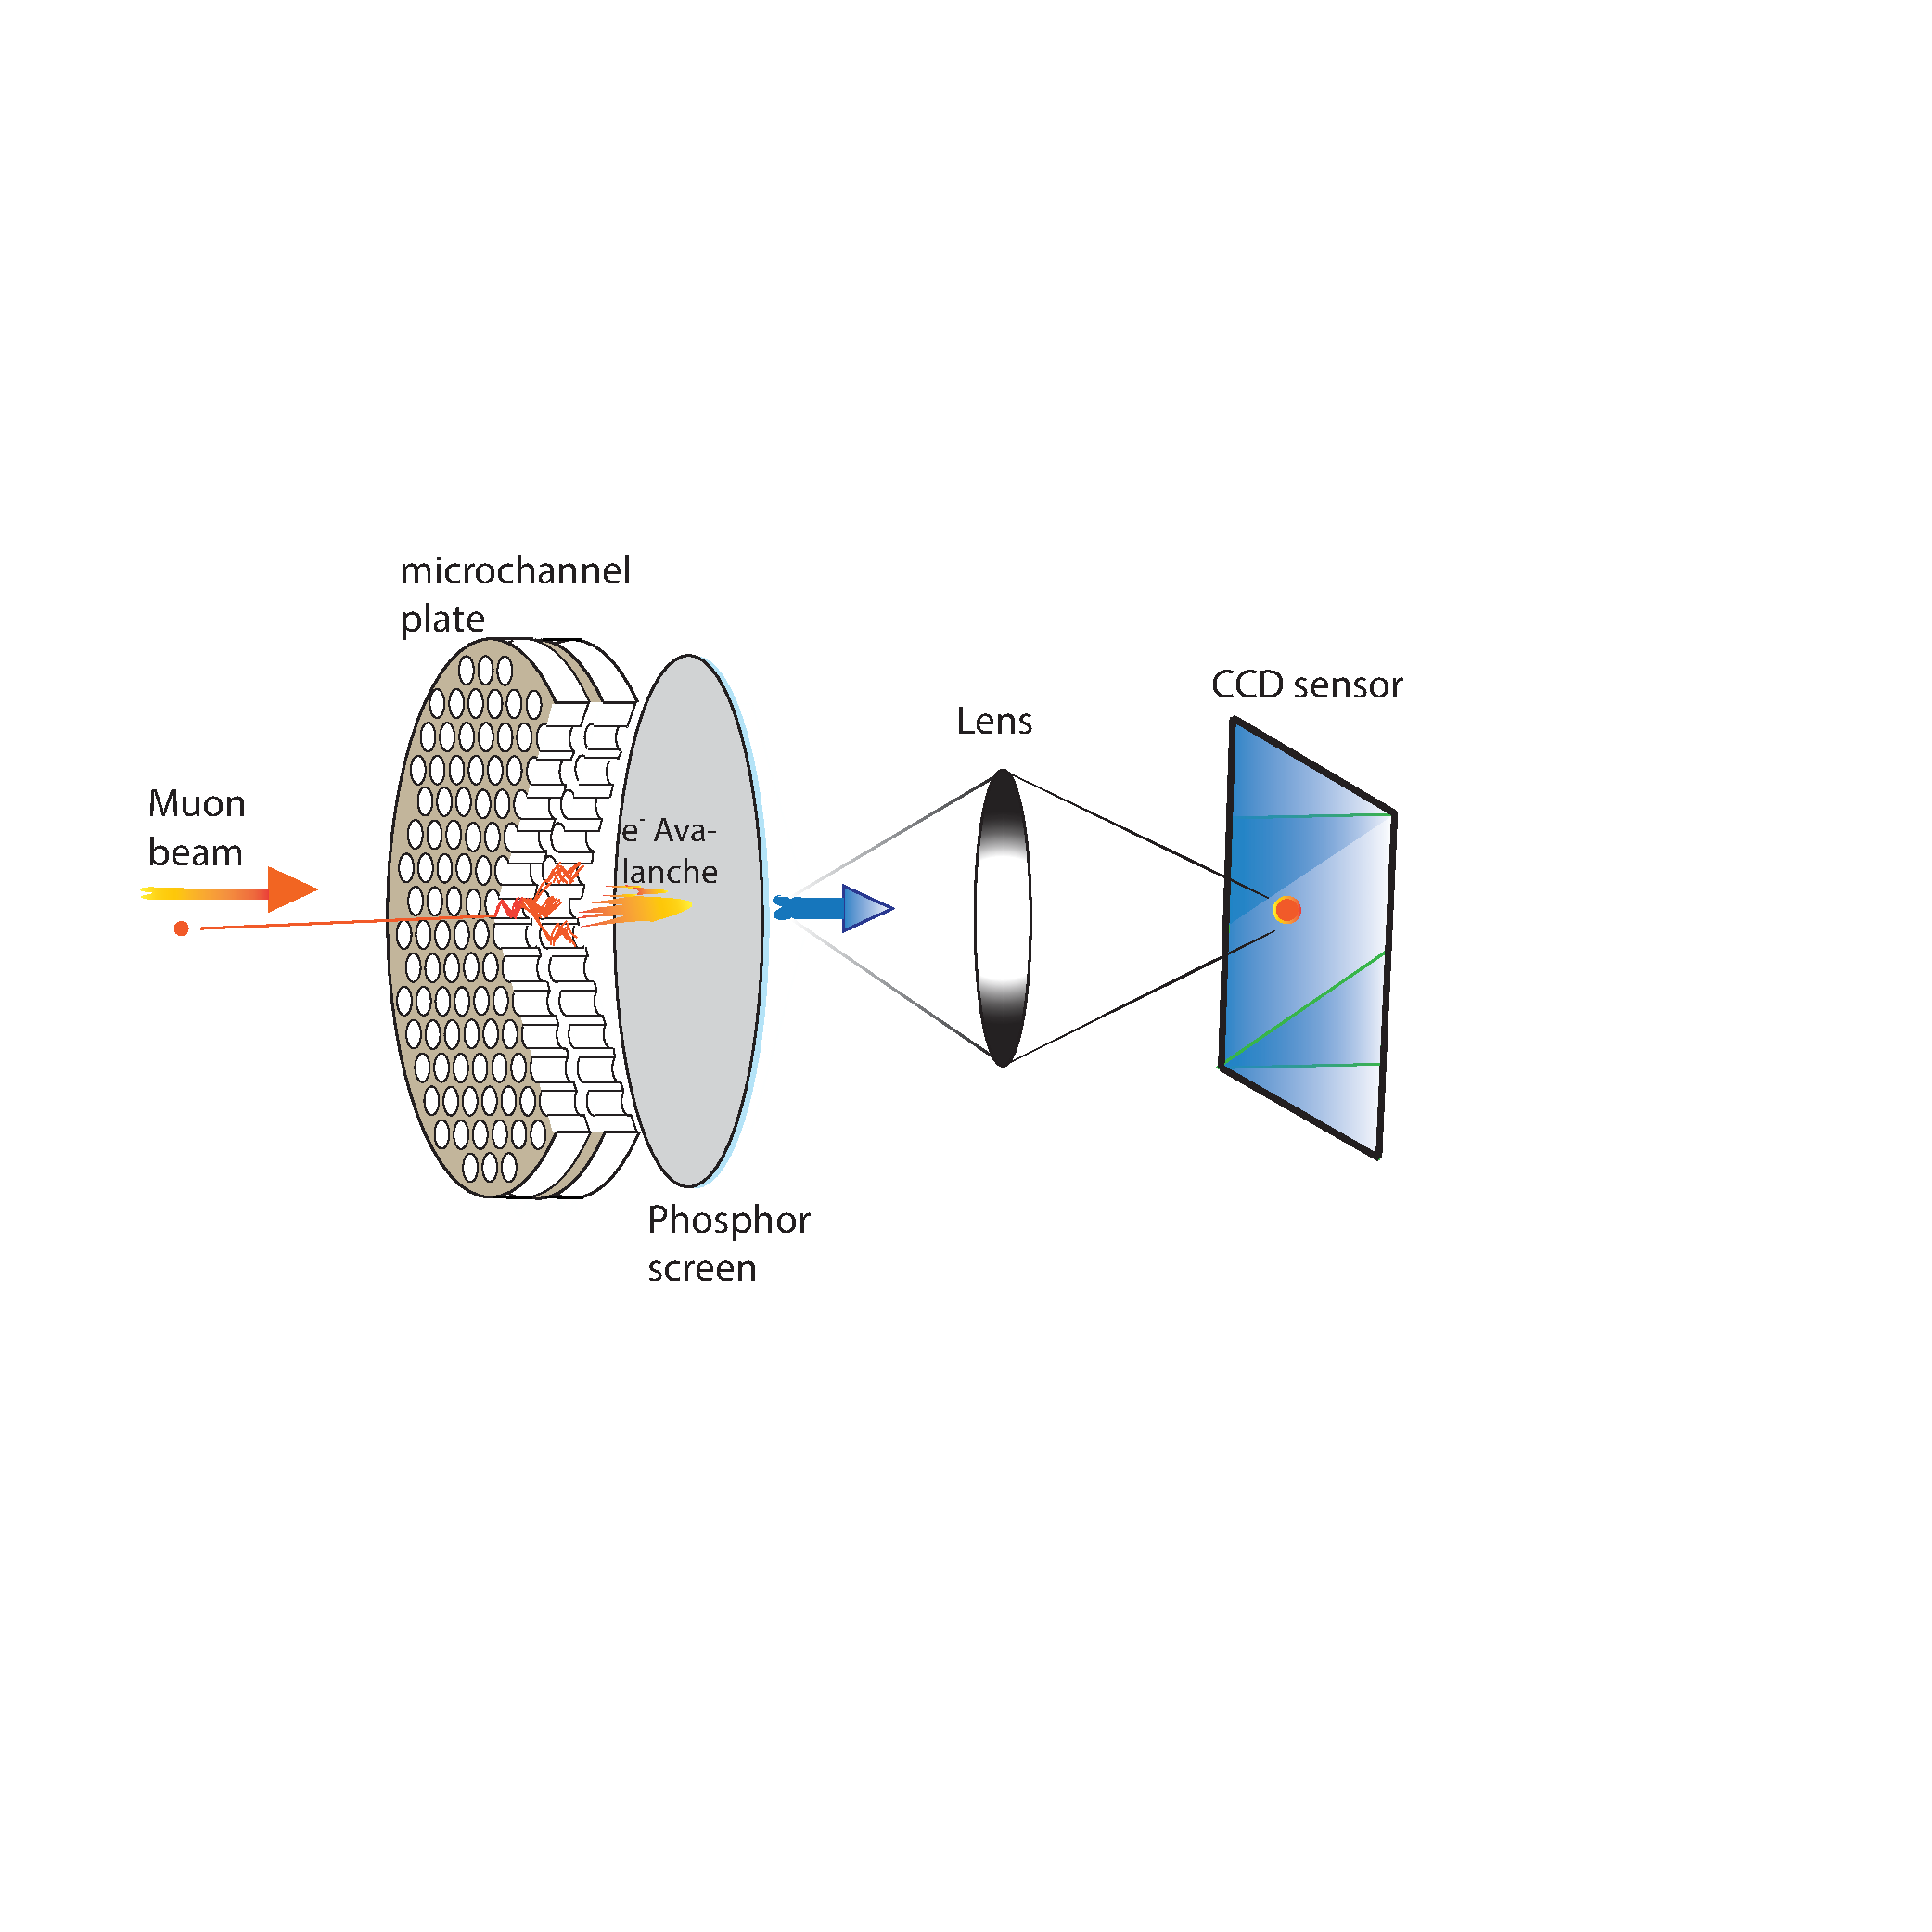
\includegraphics[width=0.6\textwidth, height=0.6\textwidth]{figure/bpm_v3.pdf}
\vspace{-3cm}
\caption{A schematic view of the BPM
}
\vspace{-0.5cm}
%\end{minipage}
\label{fig:BPM_scheme}
\end{center} \end{figure}

The MCP assembly (HAMAMATSU, F2225-21P) has two stages of chevron type MCP with an effective area of $\phi = \SI{40}{\mm}$ and a gain of $10^{6\sim7}$ and a phosphor screen (P47). The light output from the phosphor screen has been transmitted through a glass viewport (7056 Borosiliate) and then captured by the cooled CCD camera (PCO, PCO1600: $800 \times 600$ pixels for $2 \times 2$ binning mode) with the lens (ZEISS, Distagon 2/28 ZF.2). 
In order to block the electron background, negative potential (\SI{-1.9}{\kilo\volt}) is applied in the MCP front surface (MCP IN).
The MCP back surface (MCP OUT) is connected to a ground after an electric circuit to read out the electric signal of the MCP which is required to check the beam arrival time.
Positive potential (\SI{3.9}{\kilo\volt}) is applied to the phosphor screen (Phosphor IN).

An exposure time of the CCD camera is set to \SI{500}{\nano\s} to reject the positron from the muon decay ($\tau = \SI{2.2}{\micro\s}$).
The P47 phosphor material with a short decay time ($\tau_{\SI{10}{\percent}} = \SI{0.11}{\micro\s}$) compared to the exposure time has been used for this discrimination method.

The MCP assembly is installed in the middle of a cylindrical vacuum chamber constructed from stainless steel.
The MCP assembly and the CCD camera are aligned in the cylindrical axis.
The vacuum chamber has thin mylar film (\SI{0.1}{mm}) window in a flange in front of the MCP assembly for beam transmission.
Mylar film window is also in a side port for positron transmission. 
A viewport is in a flange behind the MCP assembly.

\section{Experiment with muon beam}

\subsection{Experimental setup} 

The experimental setup for the surface muon beam test is shown in Fig.\ref{fig:simulation} {(top)} and as schematic view in Fig.\ref{fig:simulation} {(bottom)}.
J-PARC facility sends surface muons ($\mu^{+}$) as pulsed beam to the MLF D2 area with \SI{100}{\nano\s} beam width, kinetic energy with \SI{4}{\MeV} and \SI{25}{\hertz} repetition rate~\cite{D-line, D-line1}.
The beam intensity is adjusted by slits in the beamline.
The beam size and intensity was adjusted by one of lead collimators with $\phi=\SI{10}{\mm}$, $\SI{20}{\mm}$ and $\SI{40}{\mm}$ hole installed between the exit window of the beam line and the BPM vacuum chamber.
The MCP assembly has been installed inside of the BPM vacuum chamber which is separated from the beam line as an independent vacuum system.

Number of muon on the BPM was measured from decay positrons.
Some fraction of the decay positrons from muons stopped in the MCP volume go through the mylar film in the left window of the BPM chamber and give signals to the positron counter. 
The positron counter consists of two plastic scintillators with corresponding light guides and PMTs. %($ch1, ch2, ch3$).
The positron counter is shielded by lead blocks from the muon beam line and the BPM vacuum chamber. This will block the decay positron from other materials and a hole of $\phi=\SI{30}{\mm}$  opened in the collimator allows positrons only coming from the MCP.
%The signal above threshold with width narrower than \SI{30}{\ns} is selected from positron counter to reject electric noise. 
%The coincidence condition between two positron counters within \SI{30}{\ns} time range is selected for decay positron from MCP region only without other background.
%A muon beam size can be larger than the effective area of the MCP by beam emittance and scattering in for large collimator hole setup.
%So some of the muon are stopped not at the MCP but at other obstacles and positrons from these muons can give signal to the positron counter. 
%Because this effect can give a bias to estimate a muon number in BPM by the positron counter, 
%The beam acceptance at the MCP with several collimator\textcolor{red}{hole sizes} %, mylar film, etc 
%is checked by the simulation.
%Also an origin of the decay positron measured in the positron counter which come from a muon stopped at the MCP or other obstacles is checked to get a correction factor for \textcolor{red}{an estimated} muon intensity from the positron counter.

\begin{figure}[tb]
{\setlength{\belowdisplayskip}{0pt}
\begin{minipage}[t]{60mm}
%\includegraphics[width=1.25\textwidth, height=1\textwidth]{figure/BPM_pic_2.pdf}
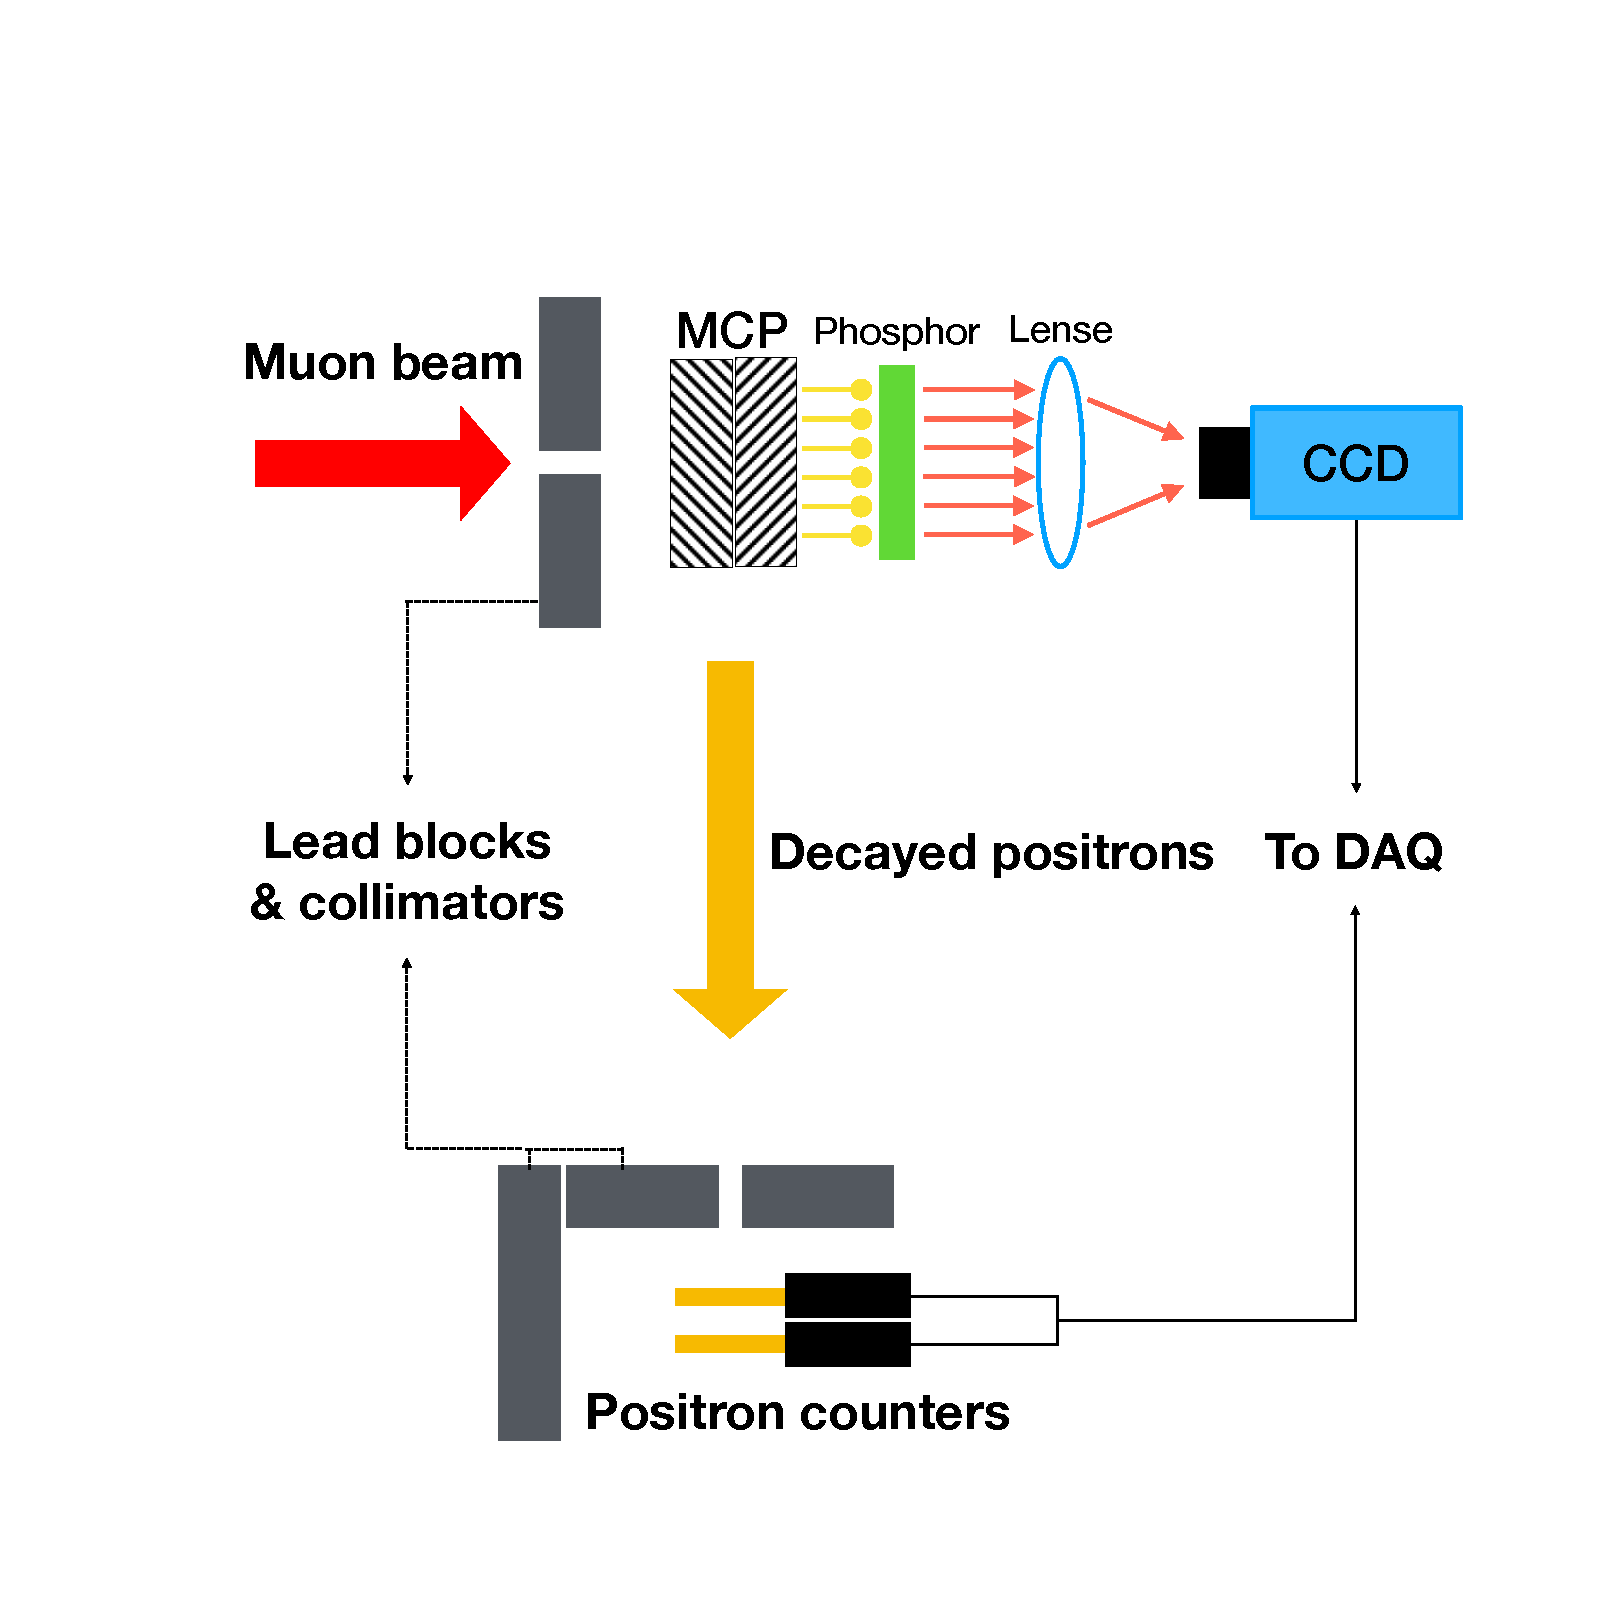
\includegraphics[width=1.25\textwidth, height=1.25\textwidth]{figure/BPM_schematic.pdf}
\end{minipage}
}
%\vspace{-0.7cm}
\caption{Setup for the test with muon beam at the J-PARC MLF D-2 line}
\vspace{-0.4cm}
\label{fig:simulation}
\end{figure}

\subsection{Data taking} 
Two dimensional pictures were taken by the CCD camera with \SI{500}{\nano\s} exposure time.
The arrival time of the muon beam has measured by the MCPOUT signal. This timing information was used 
to set the proper timing for triggering the CCD exposure. The waveform data for the positron counter has been taken for the $\SI{10}{\micro\s}$ period in coincidence with the muon beam pulse.

Data with a few muons per pulse have been taken to understand the property of single muon signal.
Then, data with higher intensities have been taken by changing the size of the slit in the beam line and collimator. 
An another set of data were taken with different trigger timing for CCD camera to understand positron signals in the BPM. %These pictures, especially with a few to several \si{\micro\s} delayed trigger timing from muon beam arrival, are taken with low intensity to high intensity.
The typical CCD image taken at different intensities are displayed in Fig.~\ref{fig:single_cluster}. The high intensity muon beam image as a raw picture (top right) and accumulation of 1000 pictures in colored histogram (top left). Low intensity muon beam raw picture is shown in (bottom left) and low intensity positron data with $\SI{2}{\micro\s}$ delayed trigger timing is shown in (bottom right).
\begin{figure}[tbp]
%	\begin{center}
	\centering
	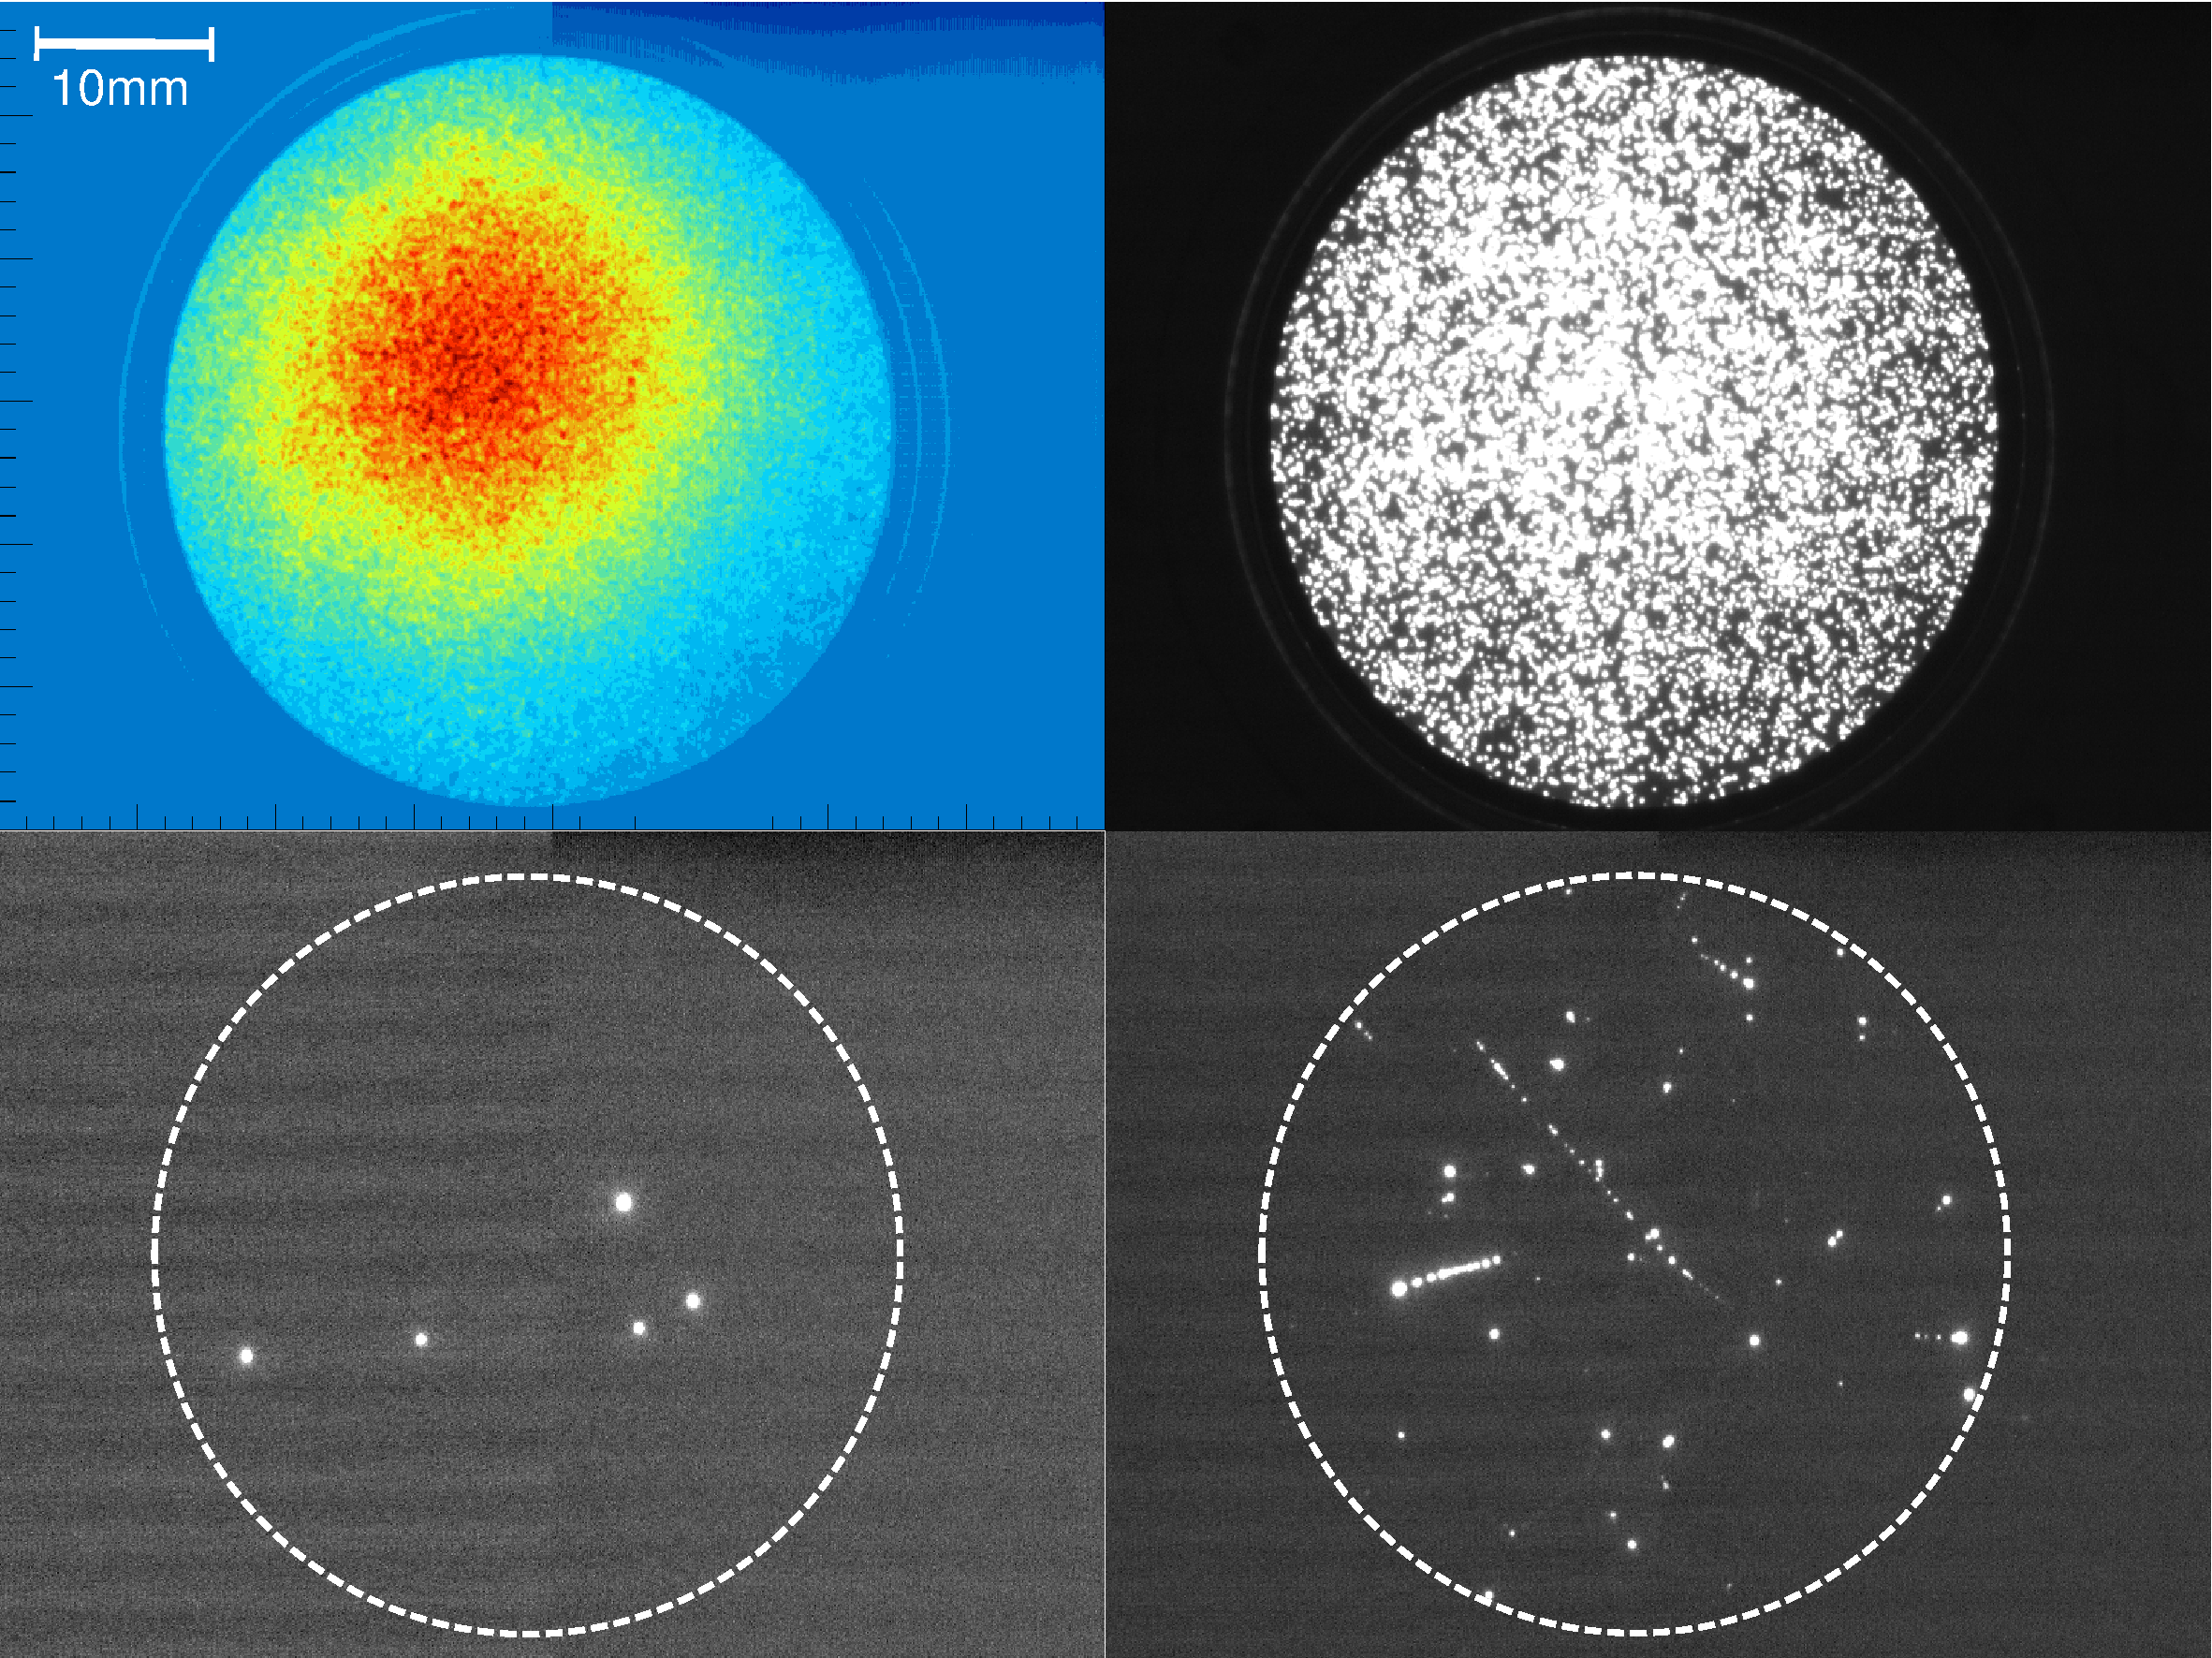
\includegraphics[width=\columnwidth]{figure/fig3_v2.pdf}
	\caption{Typical CCD images taken with muon beam. (Top left) accumulation of 1,000 pictures and (Top right) single picture at high intensity.  (Bottom left) an image taken at the muon beam timing and (Bottom right) an image of $\SI{2}{\micro\s}$ delayed trigger timing at low intensity.
	}
%	\end{center}
	\vspace{-0.4cm}
	\label{fig:single_cluster}
\end{figure}
%Even though short exposure time is used to reduce positron background, positron background is still expected in muon beam picture and this background effect is needed to be understand. 
\subsection{Data analysis}


As shown in Fig.~\ref{fig:single_cluster} (bottom left), the muon signals are distinguishable from the CCD noise by a high gain and the signal shape is a two dimensional sharp Gaussian distribution with additional broad tail distribution. 
To analyze the signals from CCD noise, a cluster is defined for single signal selection. A single cluster region for each signal is defined as $9 \times 9$ pixels from the pixel with maximum ADC count in each signal. This region is about 5 times of root mean square (RMS) width (1.6 pixel) of a single muon signal. The scale of a pixel in the picture is calculated considering the MCP active area size (\SI{0.08}{\mm \per \pixel}).

Each cluster is identified by detecting $3 \times 3$ pixels with ADC counts above some thresholds considering the standard deviation of the CCD noise fluctuation (\SI{8.7}{ADC}). The properties of single clusters are studied with this selection criteria.
%The cluster is selected from the highest ADC count while the ADC count of a pixel is above $3~\times~\sigma_{ccd}$.
%If at least 1 pixel, among 8 pixels around the maximum height pixel of a signal, has ADC count less than $1\times\sigma_{ccd}$, this signal is regarded as a CCD noise. 
%A standard deviation $\sigma_{ccd}$ of the CCD noise for each pixel are measured without beam and the value \num{8.7 \pm 0.4} ADC count is much less than the muon signal height. The properties of single clusters are studied with this selection criteria.

The distribution of the cluster ADC sum is displayed in Fig.~\ref{fig:BPM_int}.
The ADC sum distribution shows an isolated peak for exposure on muon pulse and a peakless decrease for delayed exposure ($t_{delay} = \SIlist[list-pair-separator = {, }, list-units = single]{2; 3}{\micro\s}$).

\begin{figure}[tbp]
%	\begin{minipage}[t]{60mm}
%		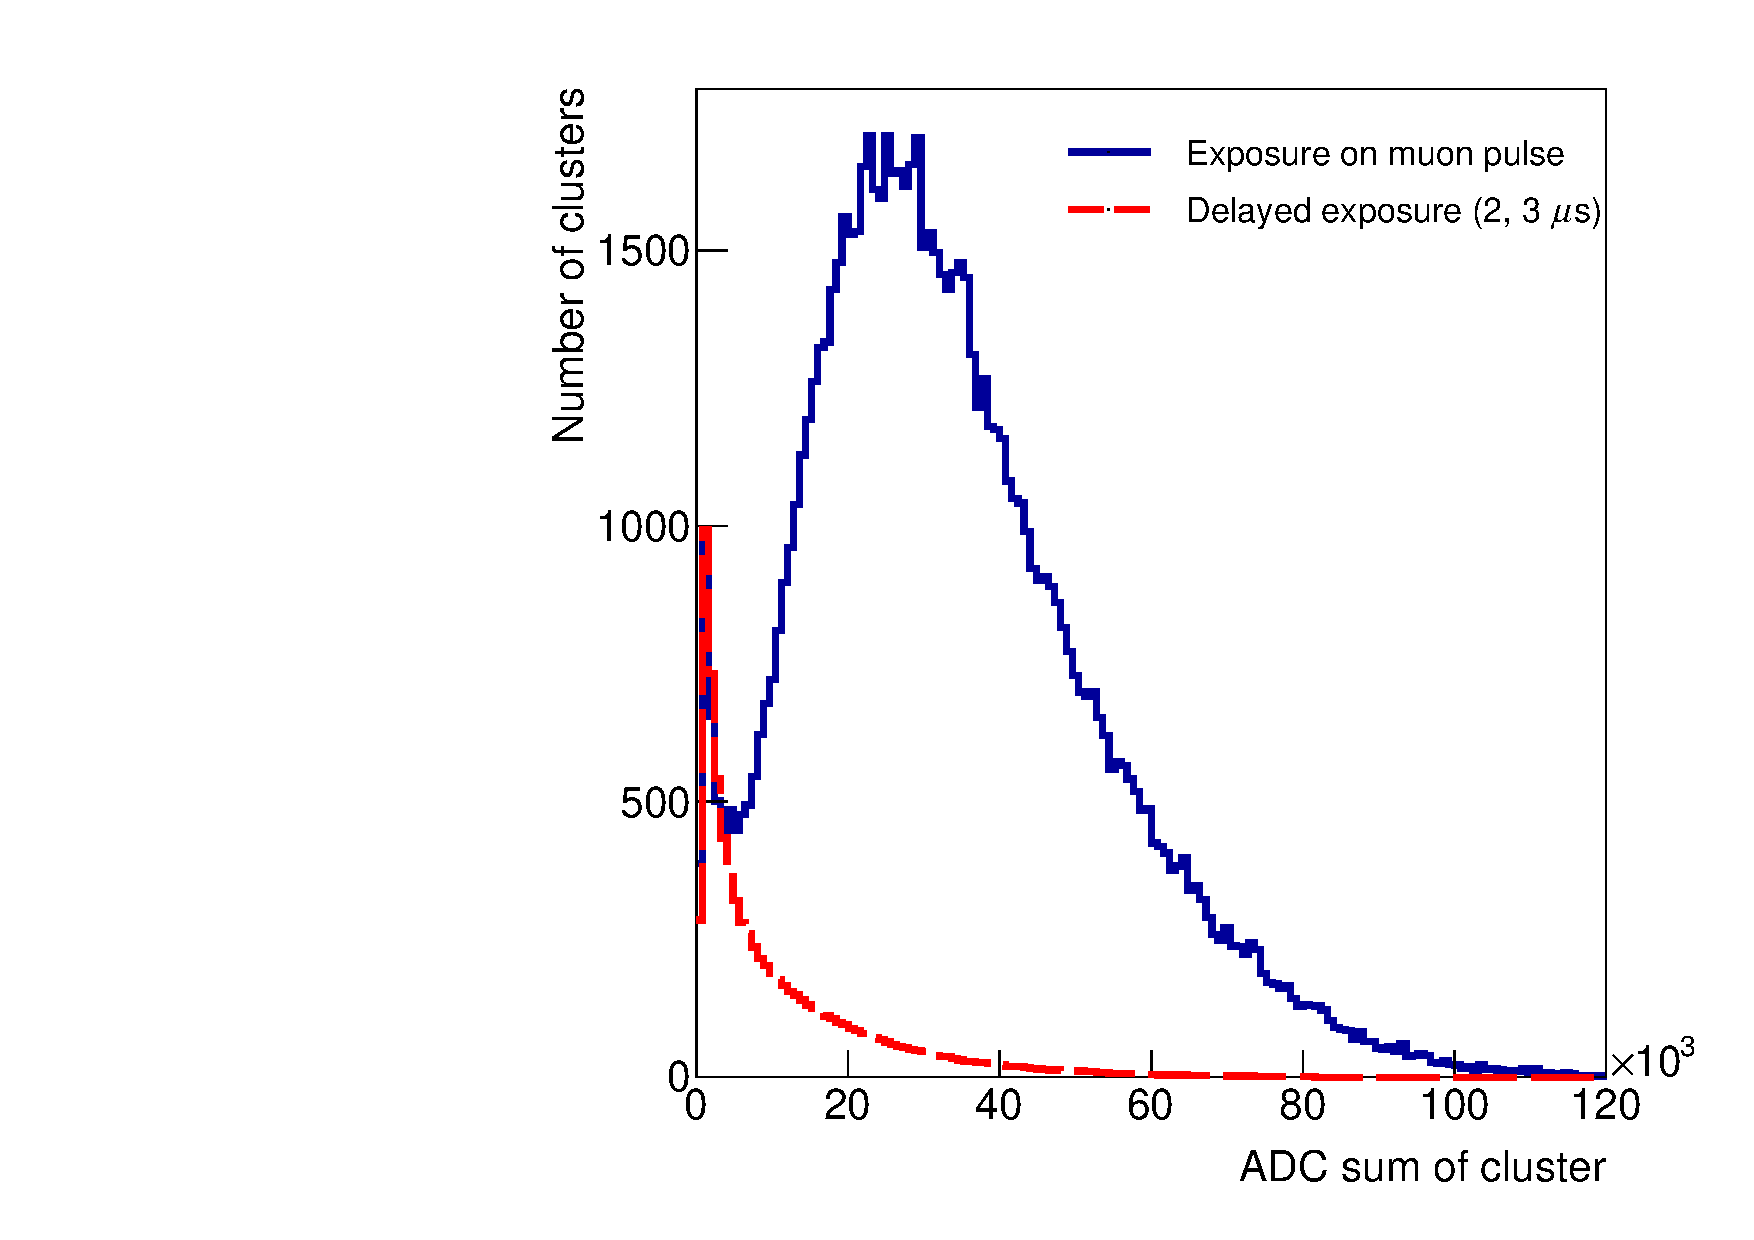
\includegraphics[width=1.30\textwidth, height=1.1\textwidth]{figure/Integ_legend_v2.pdf} %Figure4_integral_run6_7_11_9by9_sum.png}
%	\end{minipage}
	\centering
	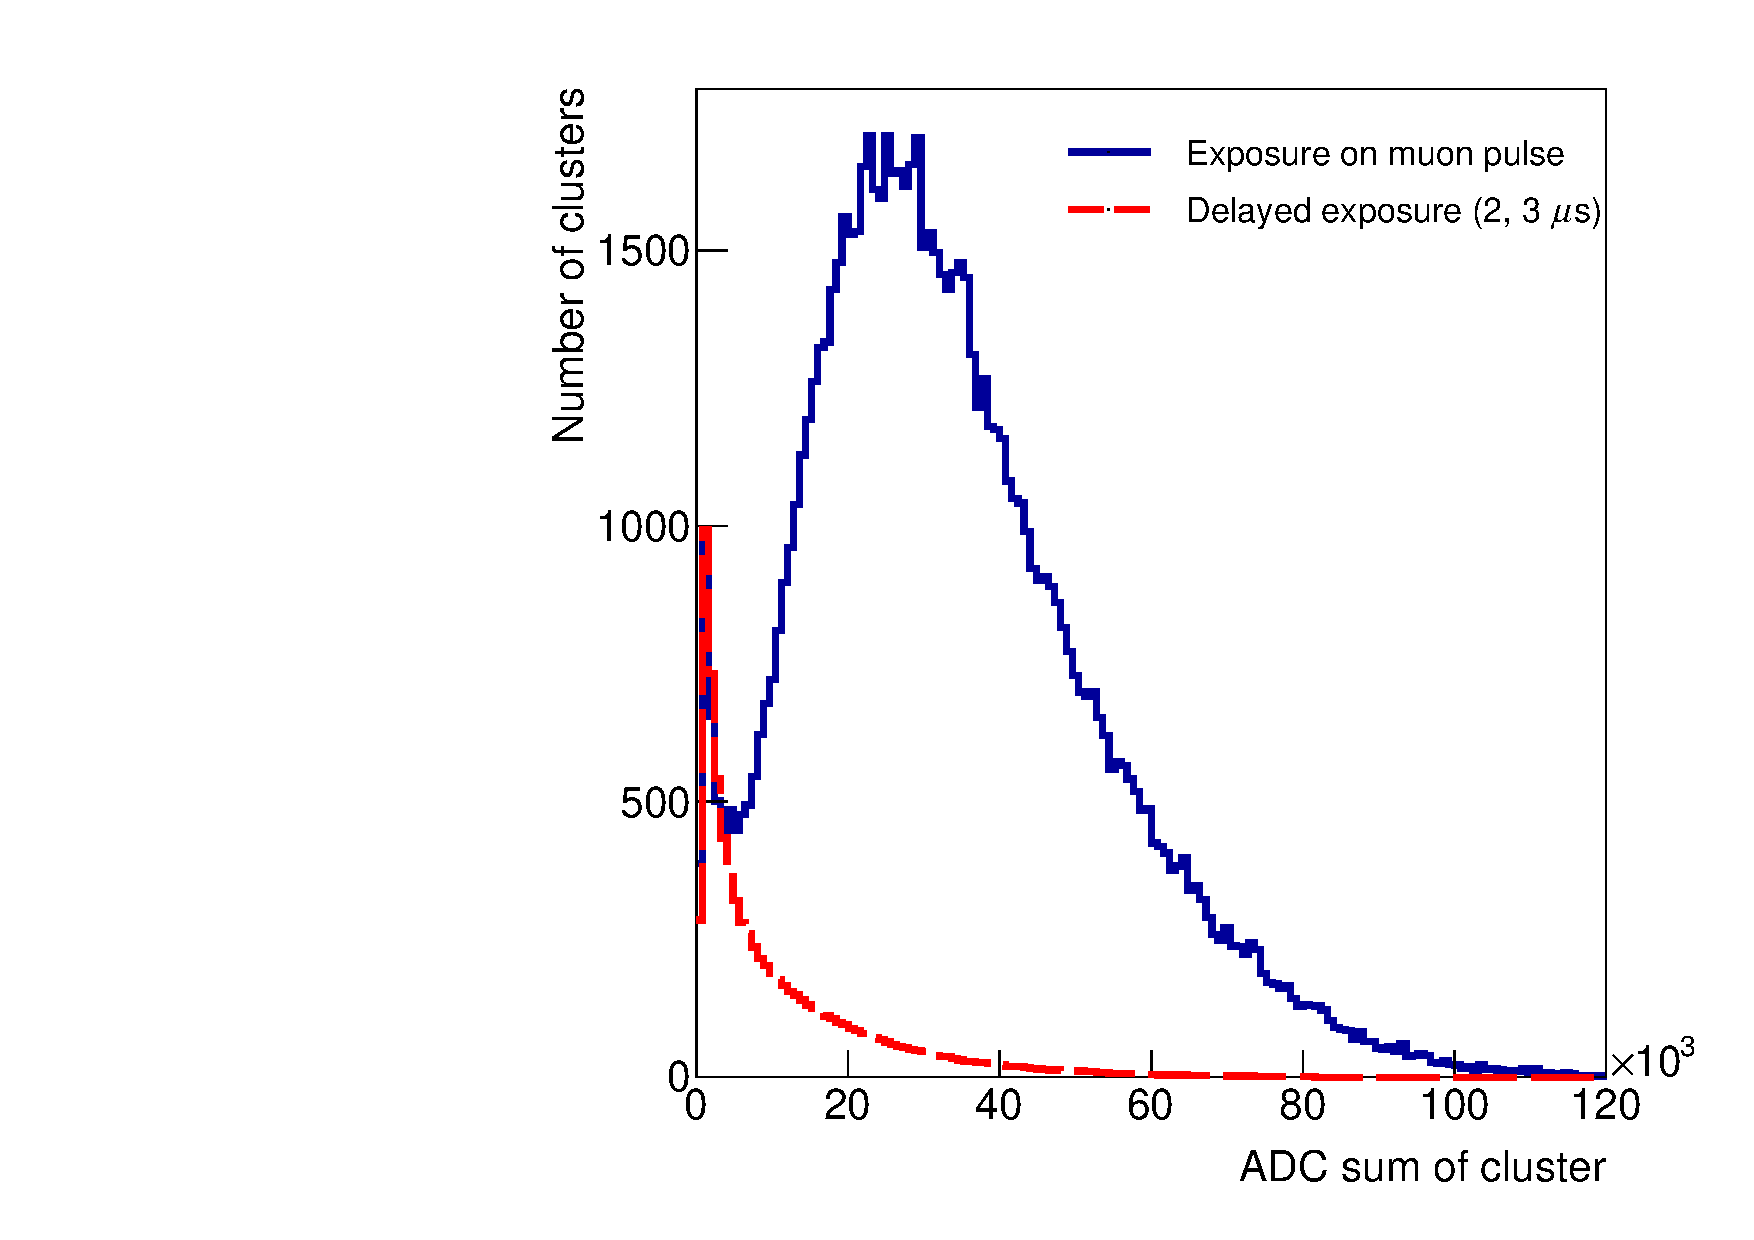
\includegraphics[width=\columnwidth]{figure/Integ_legend_v2.pdf}
	\caption{Cluster ADC sum in $9\times9$ pixels for the exposure on muon pulse (solid) and the delayed exposure (dashed).
		Normalization is done for positron histogram by matching with muon histogram}
	\vspace{-0.2cm}
	\label{fig:BPM_int}
\end{figure}

A positron signal can have an elliptic shape or even several bumps over the signal region by penetrating the MCP. That is because the decay positrons are generated inside the MCP and they have momentum with various directions. 
To parametrize the signal width, the minimum RMS width and the maximum RMS width of the clusters are calculated along the axes of each ellipse. The maximum width distribution is shown in Fig.~\ref{fig:positron_width}.

For the muon beam coincided data, the maximum width distribution is almost the same with the minimum width distribution except a small tale in maximum width distribution. This is because the incident muon has mainly longitudinal momentum and makes symmetric signal.
For the delayed exposure data
($t_{delay} = \SIlist[list-pair-separator = {, }, list-units = single]{2; 3}{\micro\s}$),
minimum width distribution is similar to that of the muon signal but maximum width distribution shows much more events with large RMS value. Under the maximum RMS width cut
($\Gamma_{max} < \SI{0.15}{\mm}$),
\SI{57}{\percent} of the clusters in delayed exposure data survive while \SI{94}{\percent} of the clusters in muon beam coincided data survive.
%the $56.8\pm0.3\%$ of positron clusters survives while $94.1\pm0.2\%$ of clusters from muon beam data survives.

\begin{figure}[tbp]
%	\begin{minipage}[t]{60mm}
%		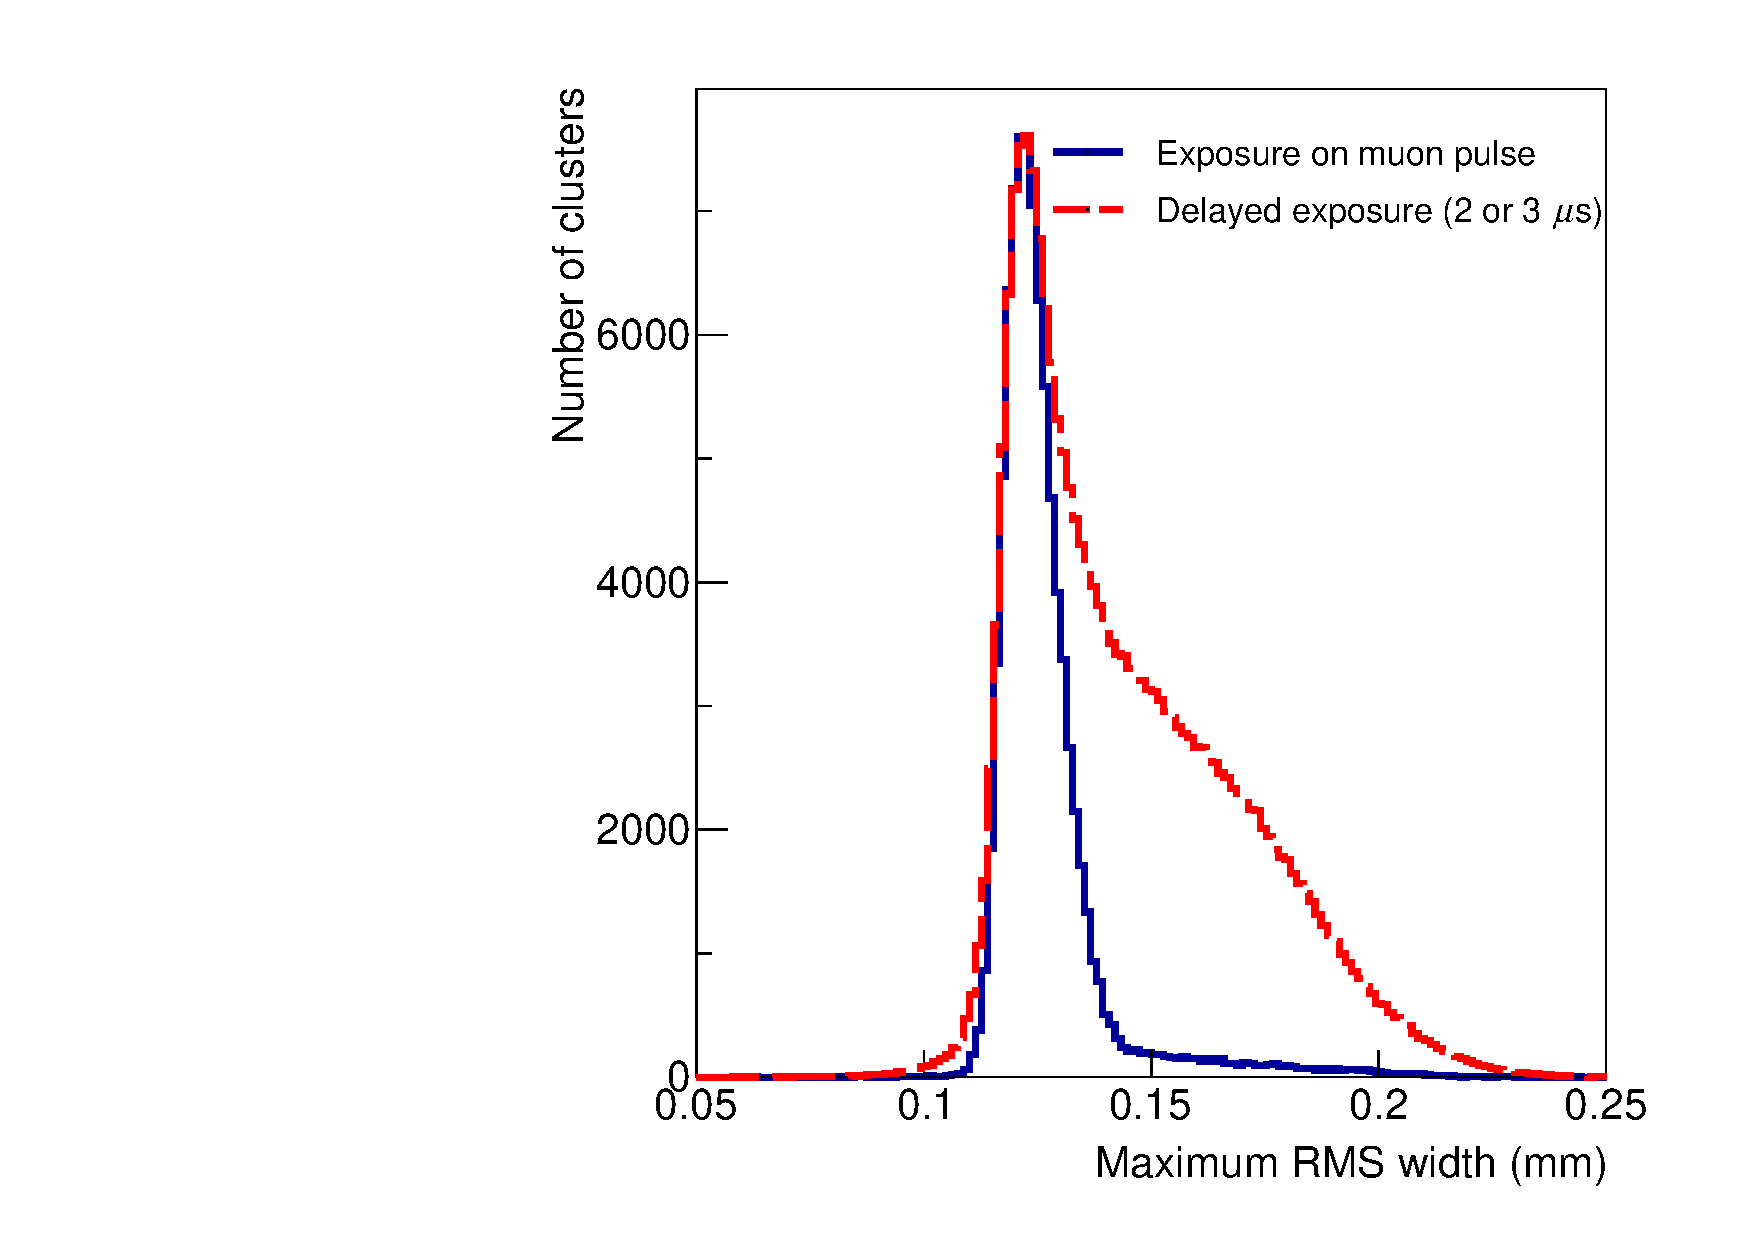
\includegraphics[width=1.30\textwidth, height=1.1\textwidth]{figure/RMS_legend_v2.pdf}
%	\end{minipage}
	\centering
	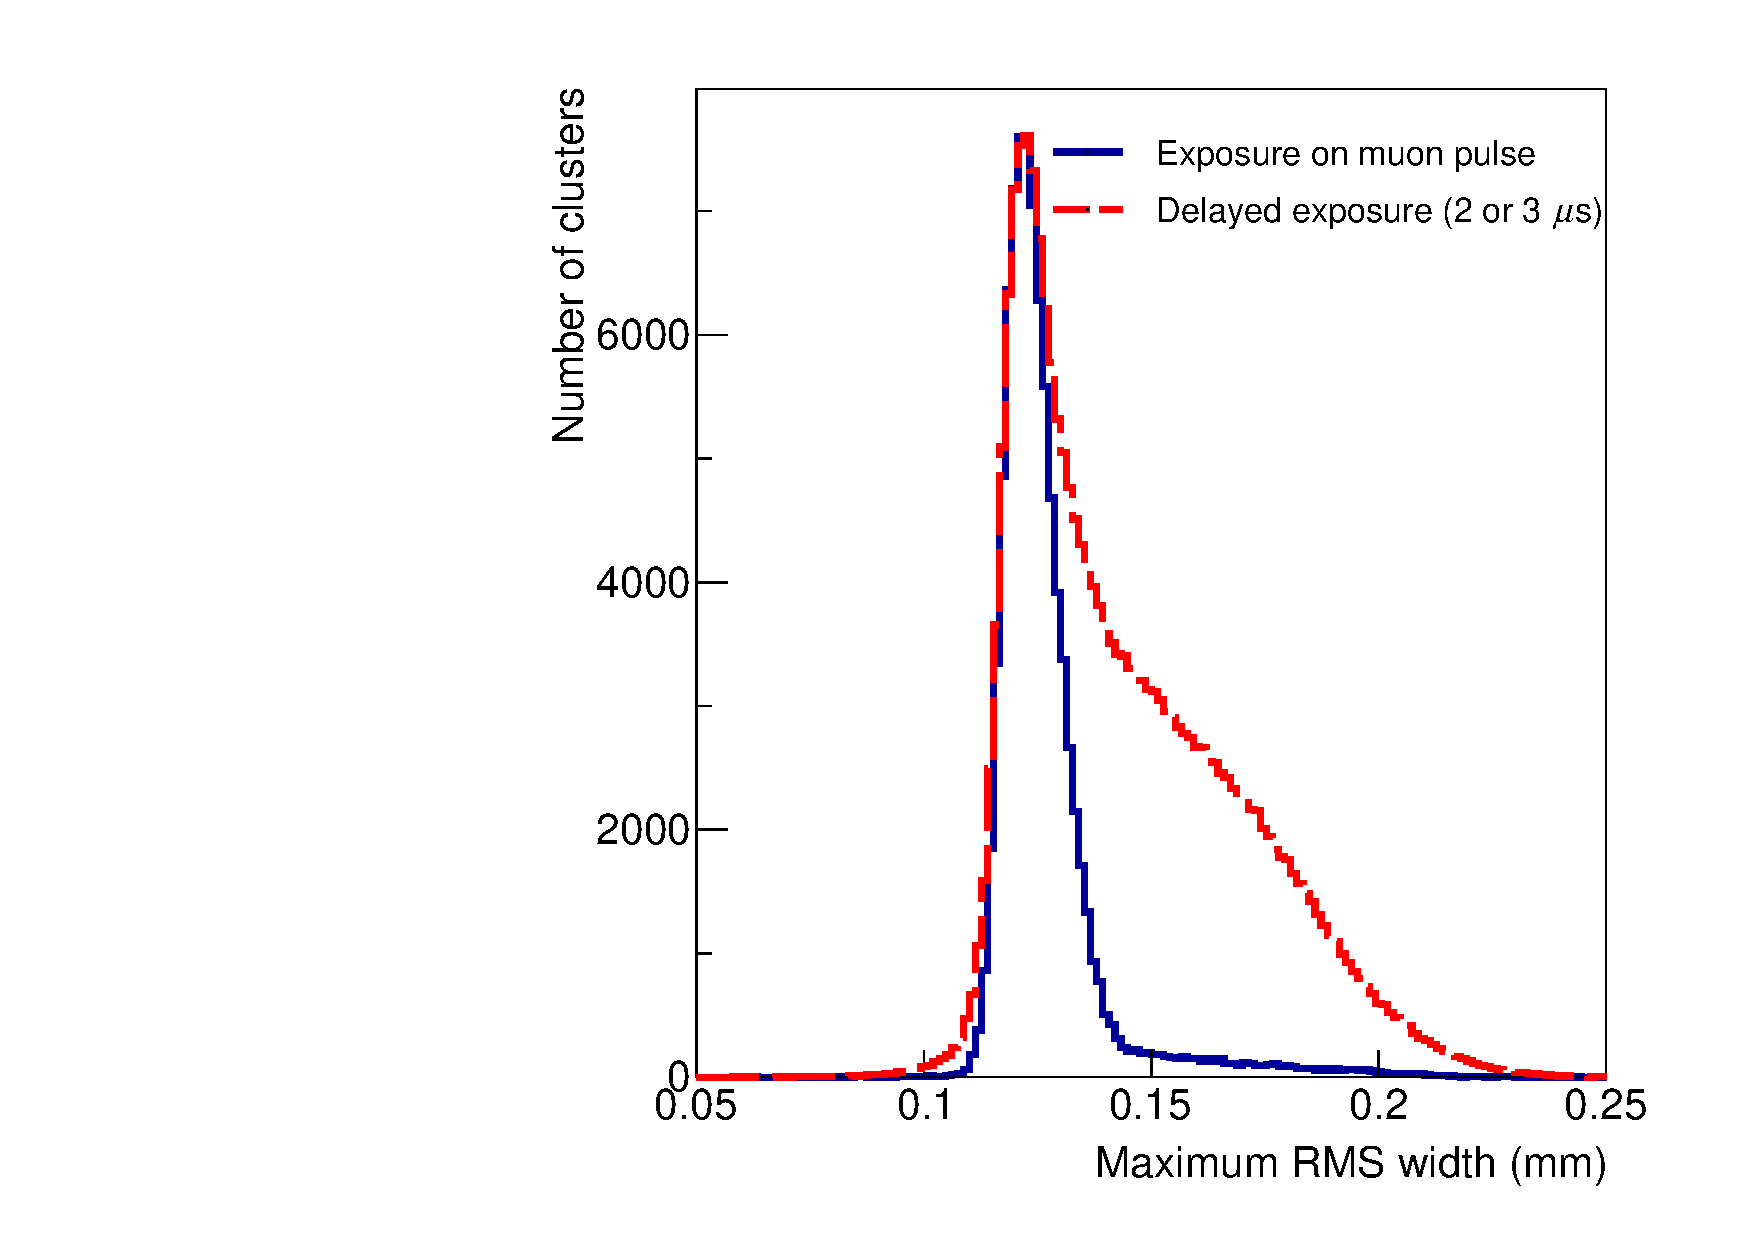
\includegraphics[width=\columnwidth]{figure/RMS_legend_v2.pdf}
	\caption{Signal's maximum RMS width histogram for the exposure on muon pulse (solid) and the delayed exposure (dashed) after rotating axes.}
	\label{fig:positron_width}
\end{figure}
%All muons which hit the MCP stop in the MCP volume. They decay into positrons and these positrons can give signals to the BPM. 
The time distribution of the decay positron is exponential decay function smeared by the time distribution of the muon beam. In order to check this distribution, the BPM data are taken by changing the trigger timing from $\SI{-0.5}{\micro\s}$ to $\SI{10}{\micro\s}$ with high intensity muon beam. The total ADC sum distribution versus the trigger time is shown in Fig.~\ref{fig:time_distribution}.

For $\SI{500}{\nano\s}$ exposure the center of which is coincided with the muon beam arrival, roughly $\SI{11}{\percent}$ of the stopped muon is expected to decay to the positron. The contribution of the decay positrons to the BPM signal is deduced from the total ADC sum distribution. The exponential function is fitted to the data in the time region later than $\SI{2}{\micro\s}$, in order to avoid the contributions of incident muons. The measured decay parameter $\tau_{\mu}=\SI{2.12 \pm 0.09}{\micro\s}$ is agreed with muon life time. The fraction of the positron contribution to the total ADC sum, $\varepsilon$, is $\SI{2.51\pm0.17}{\percent}$.

The number of muons reaching the BPM has been estimated from the total ADC sum. The necessary calibration has been obtained from the analysis of low intensity muon beam data where the response of each individual particle is identified. The average ADC count generated by single cluster, $a$, is obtained by dividing the total ADC count by the number of detected clusters in the CCD image.
\begin{figure}[btp]
%	\begin{minipage}[t]{60mm}
	\centering
	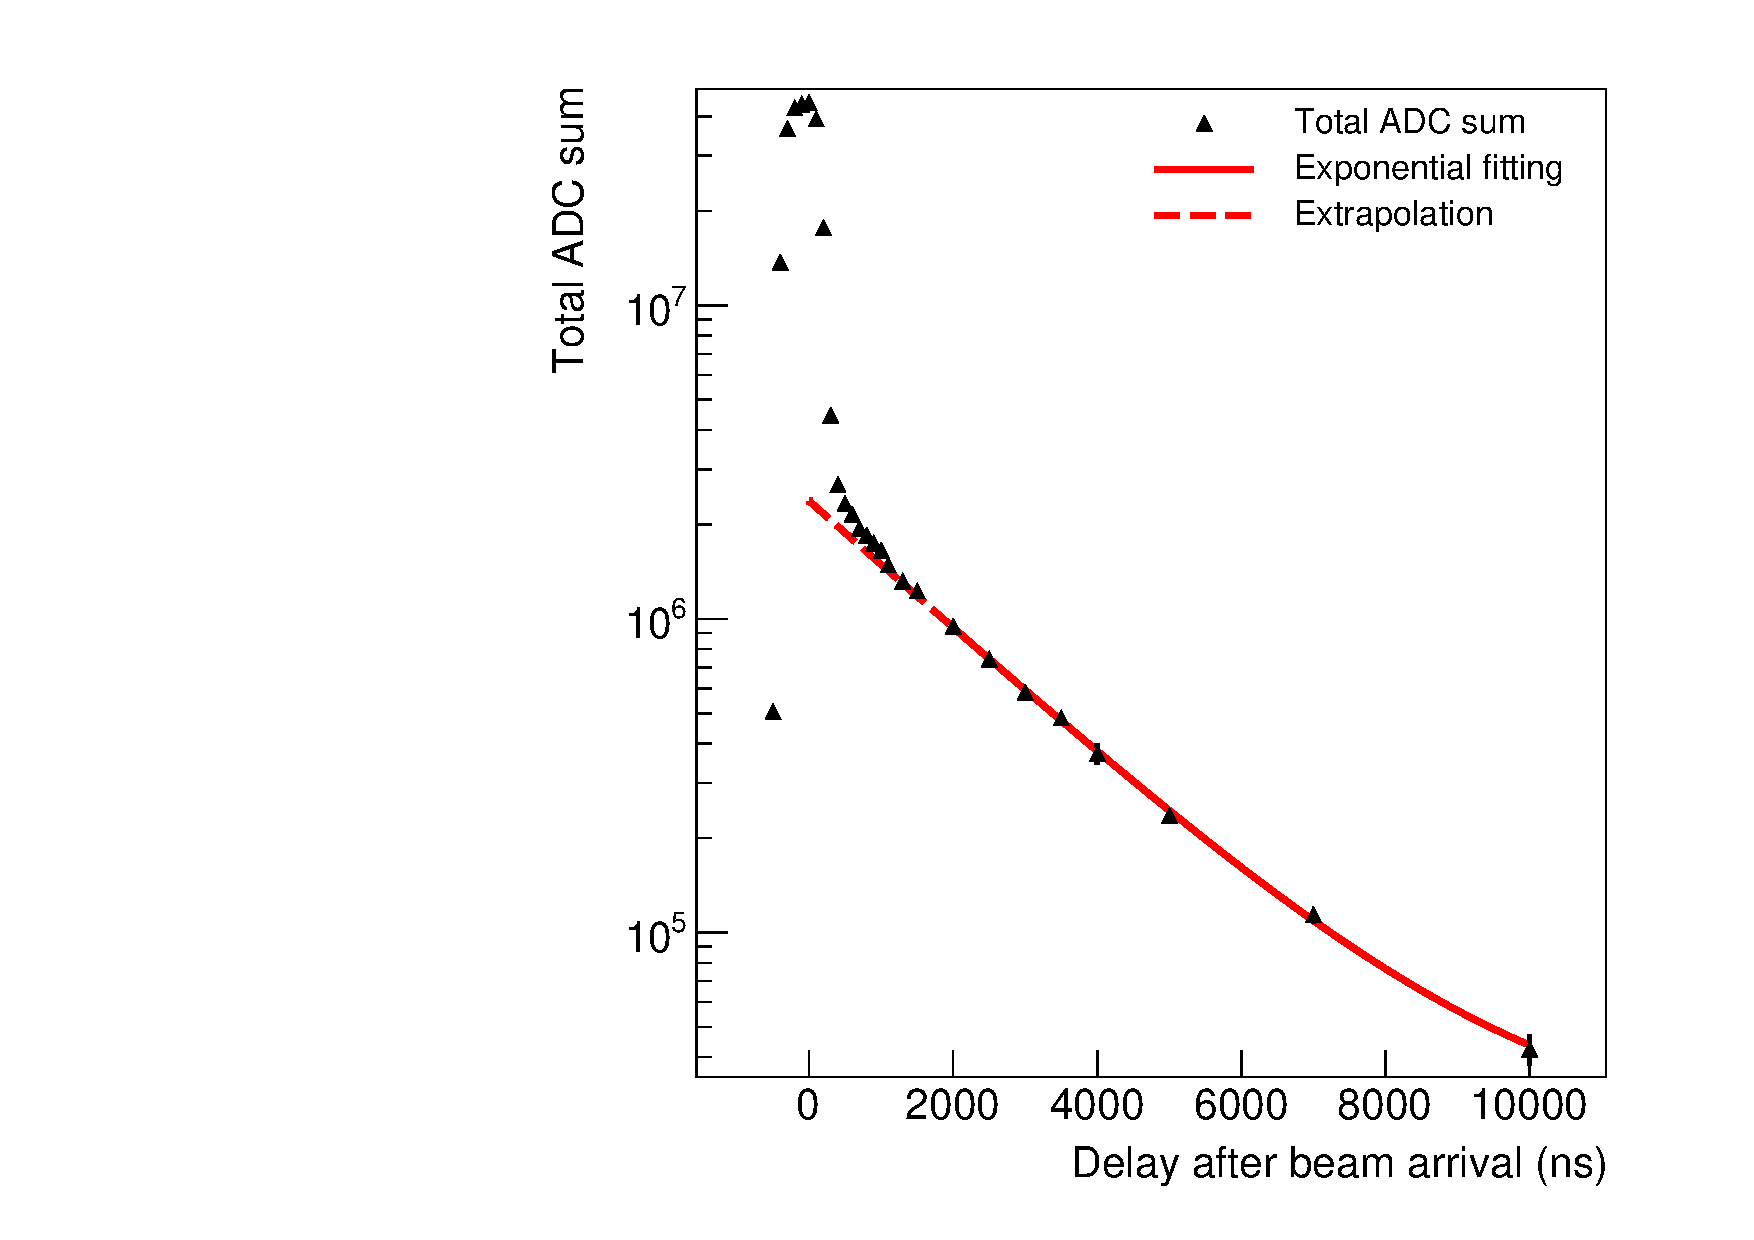
\includegraphics[width=\columnwidth]{figure/Decay_v3.pdf}
		%time_distribution.png}
%	\end{minipage}
	\caption{The time distribution of BPM signal intensity with different trigger time. An exponential function is fitted from \SI{2000}{\ns} to \SI{10000}{\ns} and extrapolation to \SI{0}{\ns} is shown.}
	\label{fig:time_distribution}
\end{figure}

The parameter $a$ from the data coincided with muon beam arrival is insufficient for the estimation of the number of muons because it contains the contributions of both muons and decay positrons. On the other hand, the data taken with enough delay from the muon beam contain contributions mostly from the positrons. By applying cluster analysis to this data, the average ADC count generated by single cluster of positron, $a_e$, is obtained. For estimating the number of positron clusters out of the total number of clusters, the $a_e$ value is used together with $\varepsilon$, the measured ADC fraction of positron signal.

For general data at various muon beam current taken in coincidence with the arrival of the beam, the total ADC sum in each picture, $A$, is measured. With the parameter $a$, the number of total clusters is calculated as $A/a$. In this way, it is possible to obtain the number of total clusters even when the single cluster is not able to be distinguished due to the high muon beam current. On the other hand, $\varepsilon A$ is considered as the ADC contribution from the positrons. Thus, the number of clusters generated by the positrons is also estimated as $\varepsilon A/a_e$. Then, the rest of clusters are considered to be generated by muons. The number of muon clusters is calculated with this reasoning.
\begin{linenomath}
\begin{equation}
C_{\mu} = C_{total} - C_{e}= A/a - A\varepsilon/a_e
\end{equation}
\end{linenomath}

It is safely assumed that one muon generates only one cluster since the transverse momentum of the muon is sufficiently limited by the upstream collimator. Therefore, the calculated number of muon clusters is taken as the number of detected muons by the BPM, $N_{\mu}$(BPM) in the $y$-axis of Fig.~\ref{fig:muvsmu}.

An another independent estimation of the number of muons is made from the number of positrons detected by the scintillators located next to the BPM chamber. The proportionality constant has been obtained from the simulation based on the actual experimental setup which is implemented in GEANT4 library \cite{geant4}. 
The simulation estimates the number of muons on the MCP from the number of positrons detected by the positron counter in coincidence with muons. 
\begin{figure}[tbp]
	\centering
	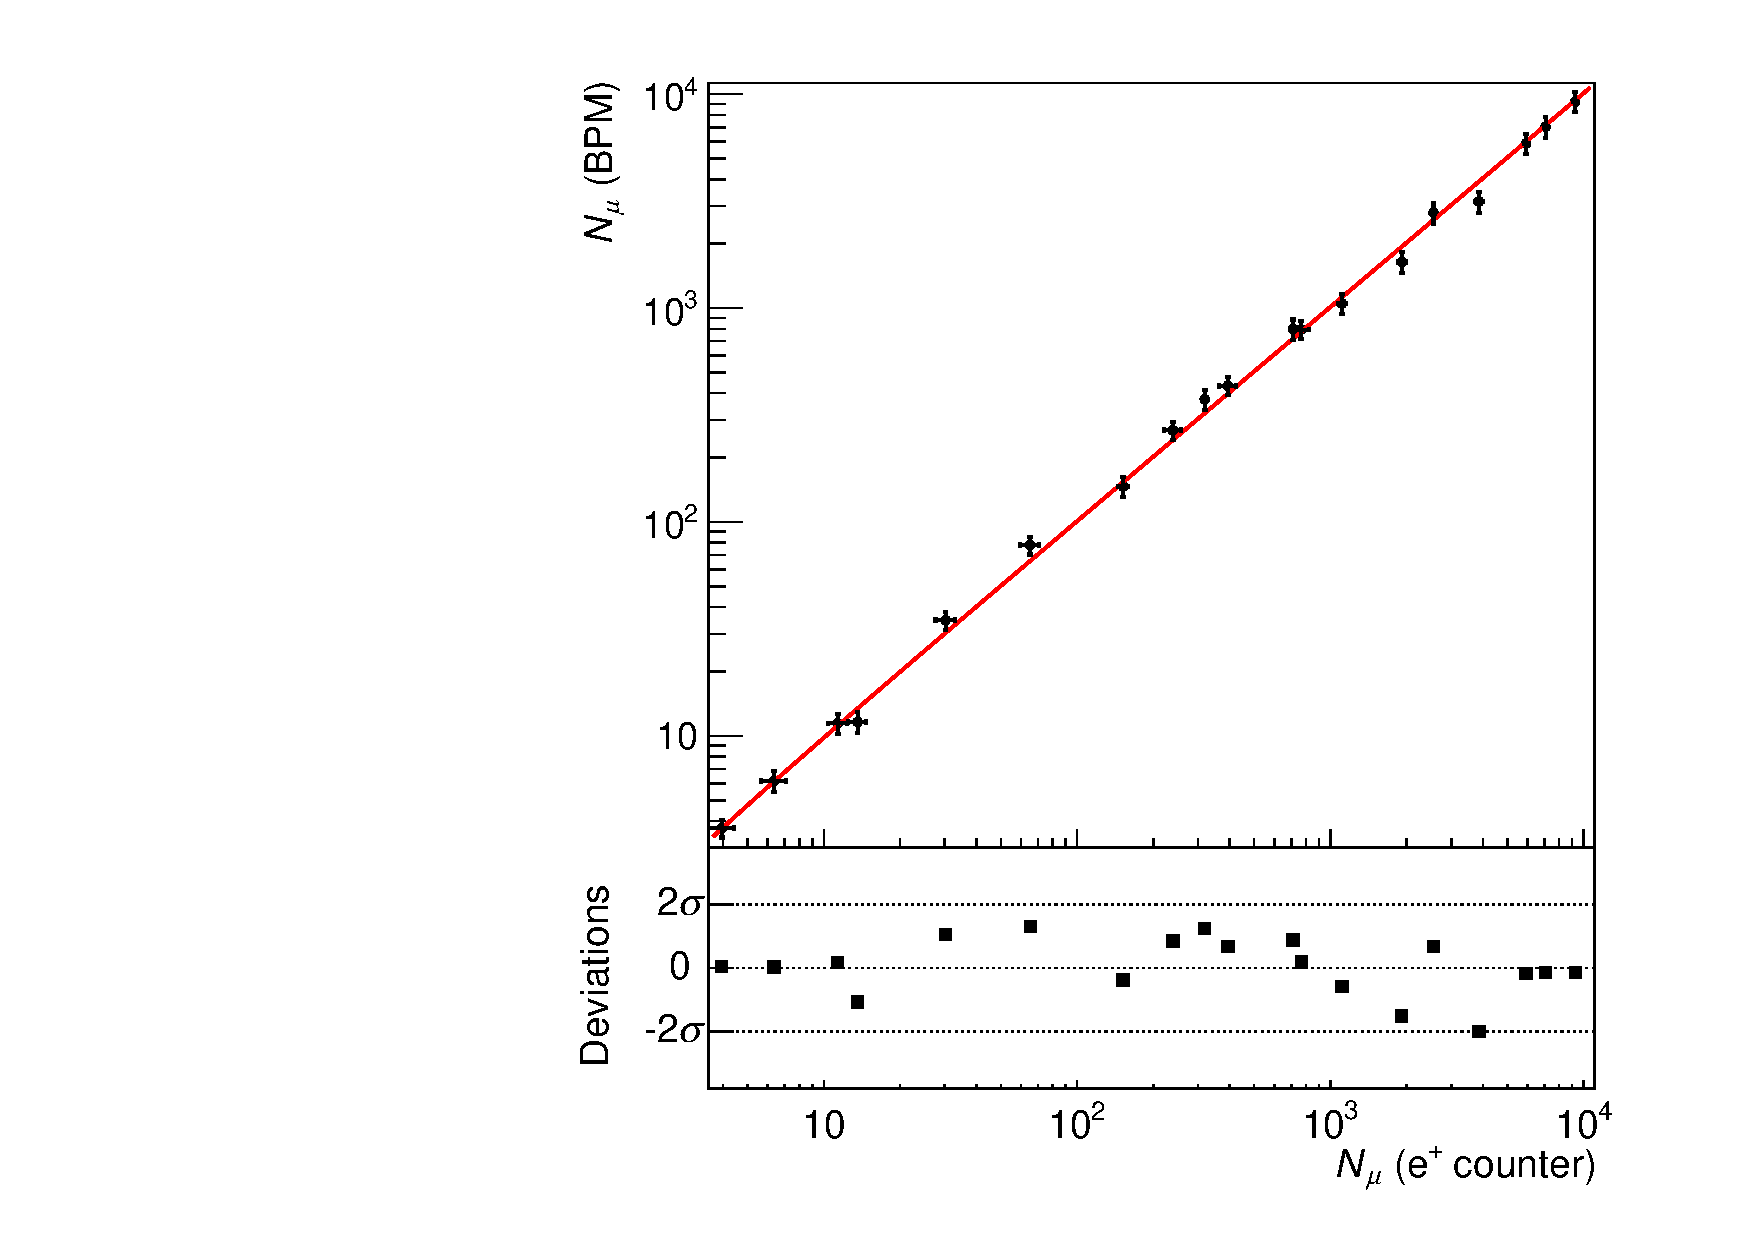
\includegraphics[width=\columnwidth]{figure/lin.pdf}
%\begin{minipage}[t]{60mm}
%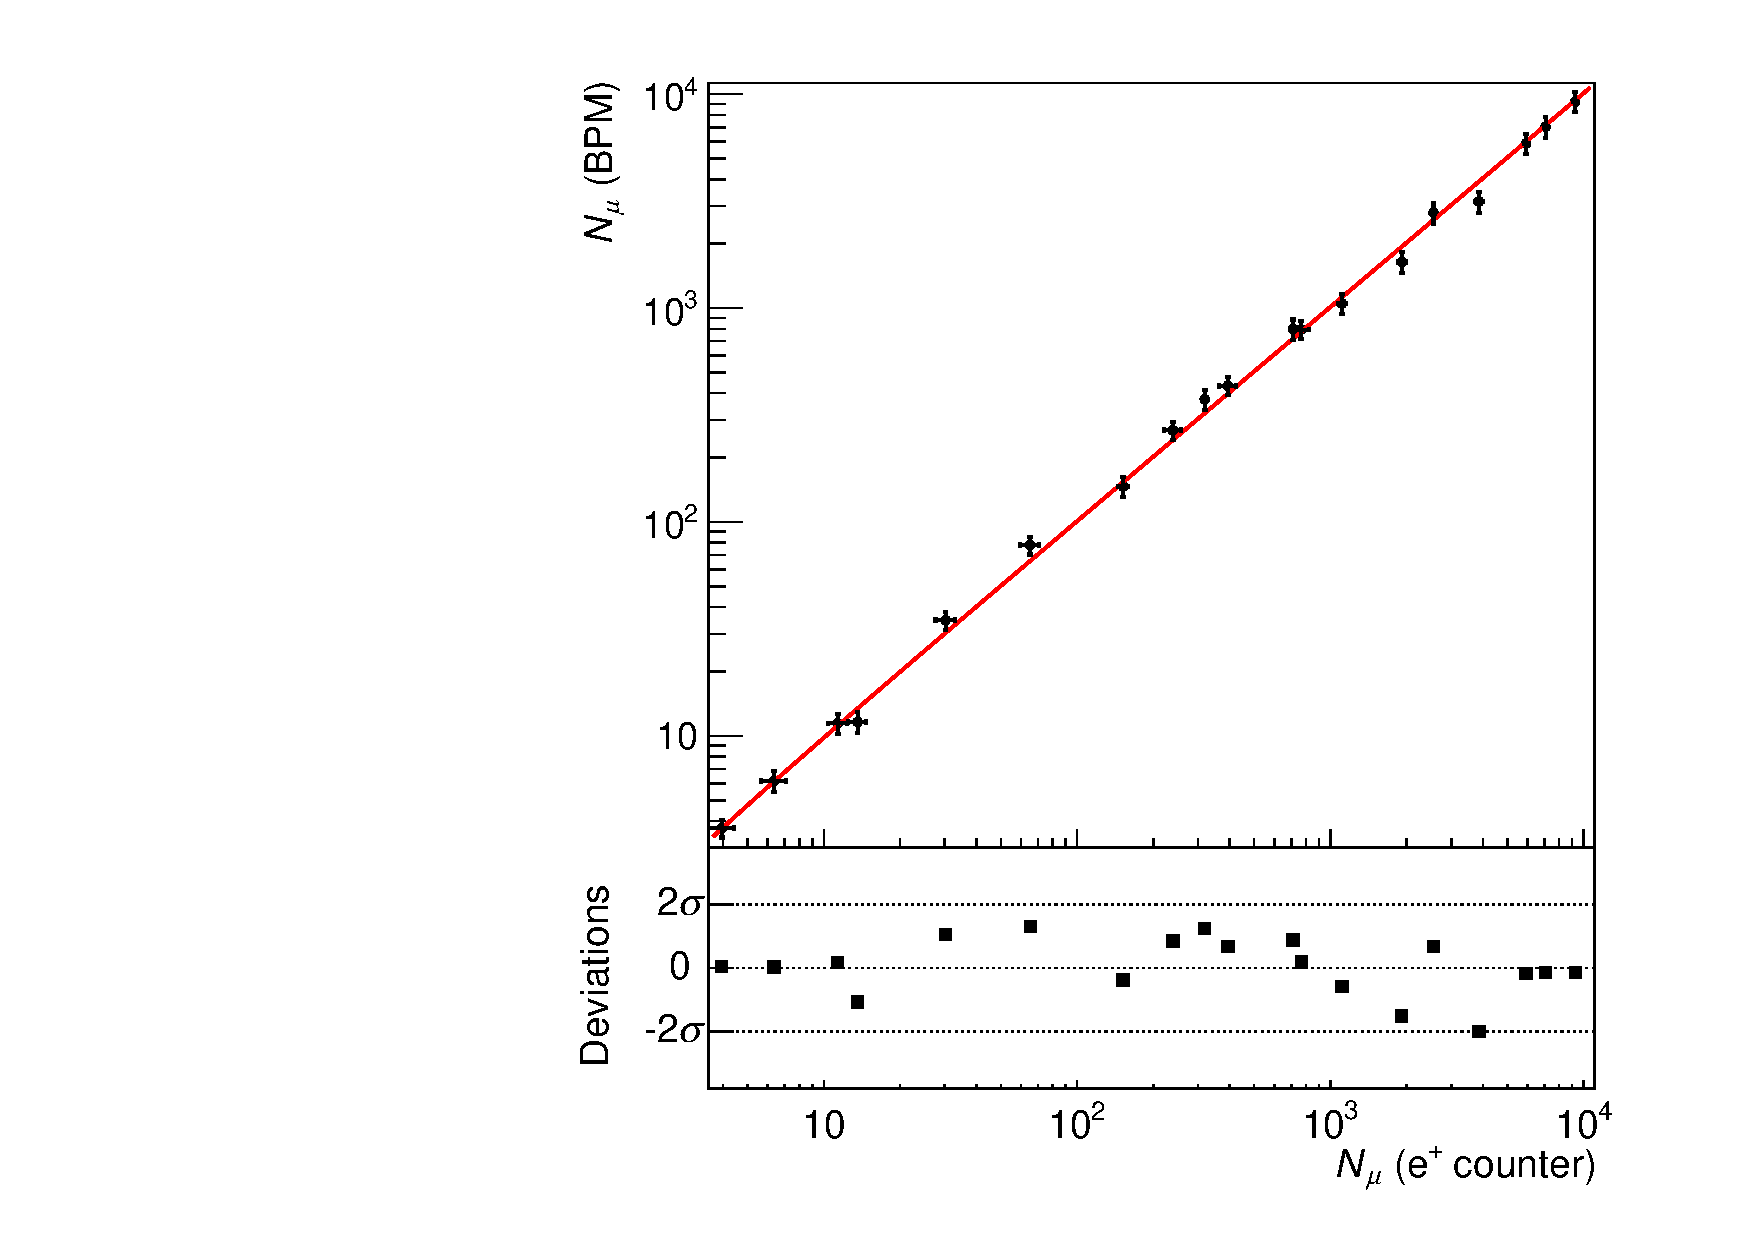
\includegraphics[width=1.3\textwidth, height=1.3\textwidth]{figure/lin.pdf}
%\end{minipage}
\caption{Estimated muon number from BPM vs estimated muon number from positron counter. 
Bottom graph shows residual distribution divided by error.}
\label{fig:muvsmu}
\end{figure}

The comparison of the number of muons obtained by these two independent methods at various values of the muon beam current is displayed on Fig.~\ref{fig:muvsmu}. The detected muon beam intensity ranges from a few muon to $10^{4}$ muon per bunch with three different size of the collimator holes and several settings of slit in the beam line.

The statistical and systematic uncertainties are considered in the errors. The major systematic uncertainties are from spatial gain difference (\SI{\sim 4.4}{\percent}), trigger timing uncertainty (\SI{\sim 3.8}{\percent}),
positron background fitting (\SI{\sim 5.6}{\percent}) and inside light reflection (\SI{\sim 2.4}{\percent}).
The statistical uncertainty is ten times smaller than systematic uncertainties except for the small positron counts in low intensity beam where the statistical error is about \SI{10}{\percent} for $N_\mu$ ($e^+$ counter).
The total error is calculated as a square root of the square sum for all contributions and it ranges from \SI{9.6}{\percent} to \SI{11.2}{\percent} for $N_\mu$ (BPM) and \SI{1.7}{\percent} to \SI{11.7}{\percent} for $N_\mu$ ($e^+$ counter) in Fig.~7.

A first order polynomial function is fitted for the whole dataset and the slope is \num{1.01 \pm 0.03}. No clear evidence of the saturation is detected and almost all measurements agreed well with fitting function within $2\sigma$.  
%with $\chi^{2}/ndf$ value of 0.87. 

\section{Spatial resolution}
 
The expected muon beam spot size at first stages of muon re-acceleration is a few millimeters.
Sharp-edge pictures were taken with a collimator and UV light source to estimate the BPM spatial resolution.
Usage of the UV light allows one to avoid the positron background inevitably related to muons.

The half-circle open \SI{.5}{\cm} thick stainless collimator was placed at \SI{1}{\cm} from the MCP front surface
such that the collimator's edge was near the MCP center.
%\textcolor{red}{\SI{0}{\nm}} photons provided by
The UV light provided by the Xe-lamp source were guided by a optical fibre to the vacuum chamber.
The light guide output is centered with the main MCP and collimator axis
with distance along this axis about \SI{15}{\cm}.
Thus the collimator cast a sharp shadow on the MCP,
the illuminated plate part gave a signal to be analyzed for estimation of the spatial resolution.

The collimator edge image was aligned to pixel rows by picture rotation and 
one pixel thick vertical slices were obtained (see Fig.~\ref{fig:half_circle}).
Discrete differentiation was applied to each slice.
The peak,
which corresponded to the location of the collimator edge,
was emphasized by Hann function multiplication.
The modulation transfer function was evaluated by the fast Fourier transformation.
The \SI{10}{\percent} height frequency $\nu_{\SI{10}{\percent}}$ was obtained using polynomial approximation to additionally suppress statistic fluctuations.
More detailed information on the UV light resolution study can be found in Ref.~\cite{Gosha}.
$\nu_{\SI{10}{\percent}}$ corresponds to $\Delta_\gamma = \SI{0.29}{\mm}$,
which should be considered as an upper limit,
because light reflection from the edge's surface induced by collimator and UV fiber misalignment.

\begin{figure}[tbp]
    \centering
	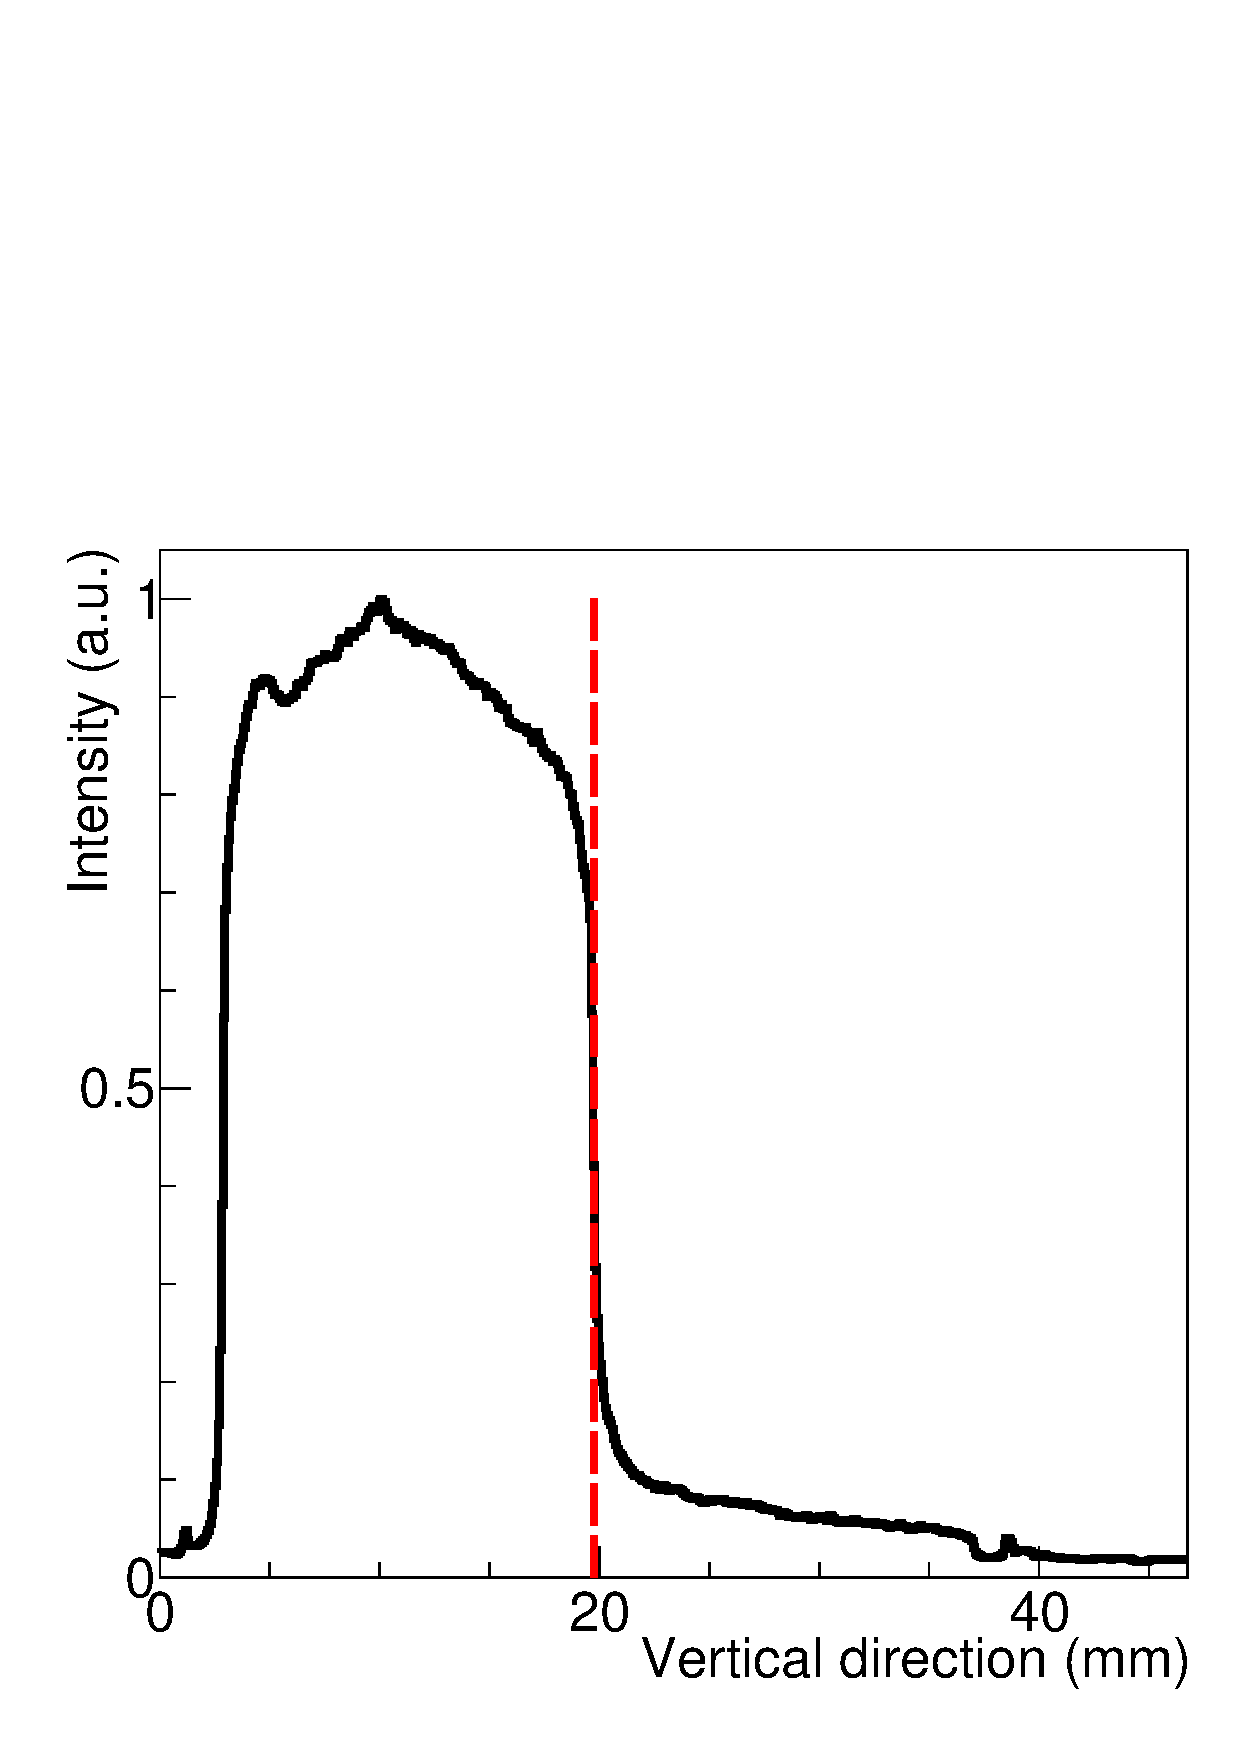
\includegraphics[width=\columnwidth]{figure/edge_image_w_uv_4_BH_axis.pdf}
	\caption{Projected ADC count distribution to Y-axis after proper rotation for UV light data with half circle collimator.}
	\label{fig:half_circle}
\end{figure}

The spatial resolution upper limit for muons is considered to be the same as well the signal from single particles has almost equal widths
$\sigma_{\mu} / \sigma_{\gamma} = \num{1.04 \pm 0.10}$.
Such a resolution satisfies the accelerator requirements.


\section{Conclusion}

A BPM has been developed measure the profile of  the ultra-cold muon beam 
for the J-PARC muon $g-2$/EDM experiment. 
The BPM has been tested and evaluated by a surface muon beam and a UV light source.
A spatial distribution of muon beam with this BPM was measured with
a high signal to background ratio between muon signals and positron.
The positron background rate has been reduced to a negligible level with 
a short exposure window for CCD camera and the additional selection on the CCD image.
A good linearity was confirmed without noticeable saturation from a few muons to \num{e4} muons.
The spatial resolution was estimated as less than \SI{.30}{\mm} from the UV light data.
%All test is well agreed with designed BPM requirements.

%This study can be a good reference for a low energy and low intensity beam diagnostics like anti-proton or positron beam which is well developed recently.
%The anti-proton or positron beams decay or annihilate to detectable daughter particles in beam profile monitor and our BPM study would be helpful to understand signal in the detector.

\section*{Acknowledgmens}

We are grateful to the J-PARC personal for the excellent machine operation.
We thank Dr. T.U~Ito for his advice on the technical design. This work was supported by 
the JSPS KAKENHI Grant Numbers JP26287053, JP15H03666, JP16J07784,
the Korean National Research Foundation grants NRF-2015K2A2A4000092, NRF-2015H1A2A1030275, NRF-2017R1A2B3007018,
the Russian Foundation for Basic Research grant RFBR 17-52-50064 and
the Russian Science Foundation grant RNF-17-12-01036,
Japan-Russia Research Cooperative Program.

\section*{References}

\bibliography{mybibfile}

\end{document}